\documentclass{article}
\usepackage[a4paper, top=2cm, bottom=2cm, left=2.5cm, right=2.5cm]{geometry}
\usepackage{graphicx}
\usepackage{float}
\usepackage{amsfonts}
\usepackage{amsmath}
\usepackage{listings}
\usepackage{xcolor}
\usepackage[dvipsnames]{xcolor}
\usepackage[normalem]{ulem}
\usepackage{hyperref}

\lstdefinestyle{htmlstyle}{
    language=HTML,
    backgroundcolor=\color{gray!10},
    basicstyle=\ttfamily\small,
    keywordstyle=\color{blue},
    tagstyle=\color{black},
    stringstyle=\color{green!60!black},
    commentstyle=\color{gray},
    numbers=left,
    numberstyle=\tiny\color{gray},
    stepnumber=1,
    numbersep=5pt,
    breaklines=true,
    tabsize=2,
    showstringspaces=false
}

\lstdefinelanguage{JavaScript}{
  keywords={typeof, new, true, false, catch, function, return, null, catch, switch, var, if, in, while, do, else, case, break},
  keywordstyle=\color{blue}\bfseries,
  ndkeywords={class, export, boolean, throw, implements, import, this},
  ndkeywordstyle=\color{darkgray}\bfseries,
  identifierstyle=\color{black},
  sensitive=false,
  comment=[l]{//},
  morecomment=[s]{/*}{*/},
  commentstyle=\color{purple}\ttfamily,
  stringstyle=\color{red}\ttfamily,
  morestring=[b]',
  morestring=[b]"
}

\lstset{
   language=JavaScript,
   backgroundcolor=\color{gray!10},
   extendedchars=true,
   basicstyle=\footnotesize\ttfamily,
   showstringspaces=false,
   showspaces=false,
   numbers=left,
   numberstyle=\footnotesize,
   numbersep=9pt,
   tabsize=2,
   breaklines=true,
   showtabs=false,
   captionpos=b
}

% Titolo
\title{Appunti di Linguaggi e Tecnologie per il Web}
\author{Federico Falcone}
\date{\today}


\begin{document}

\maketitle
\tableofcontents
\newpage

\section{Networking}
\subsection{Topologie}
Ogni tipologia di rete può essere fisicamente realizata sfruttando topologie differenti:
\begin{itemize}
    \item topologia logica a Bus, cablata a stella
    \begin{figure}[H]
        \centering
        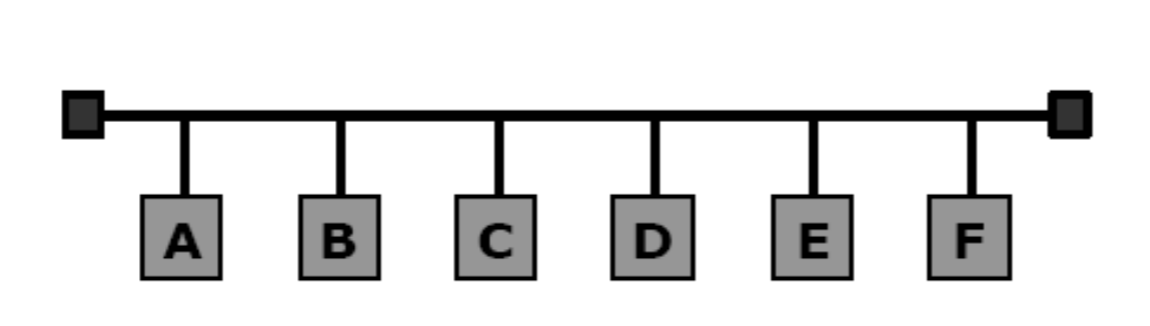
\includegraphics[width=0.4\textwidth]{Images/bus_lineare.png}
    \end{figure}
    \item topologia a stella
    \begin{figure}[H]
        \centering
        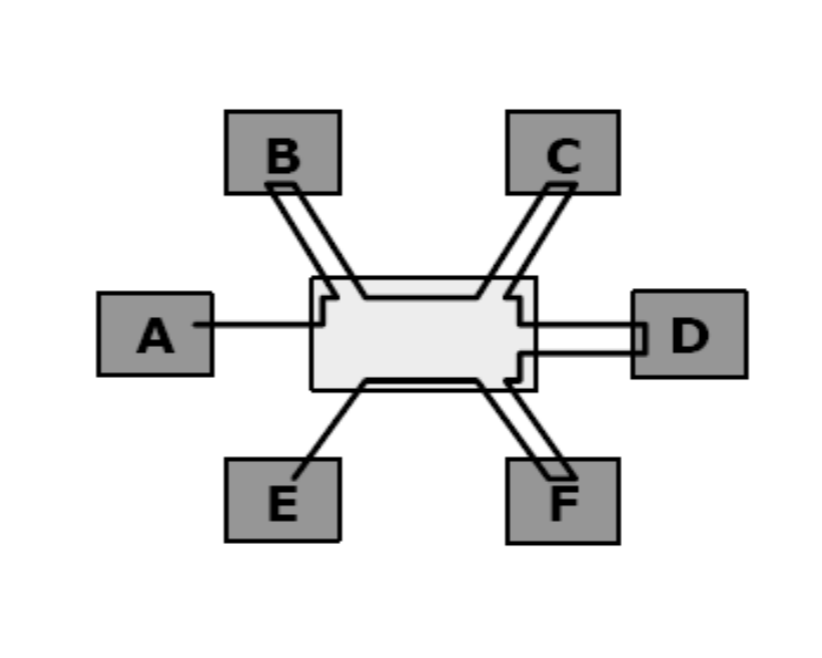
\includegraphics[width=0.4\textwidth]{Images/bus_stella.png}
    \end{figure}
    \item centralizzata
    \begin{figure}[H]
        \centering
        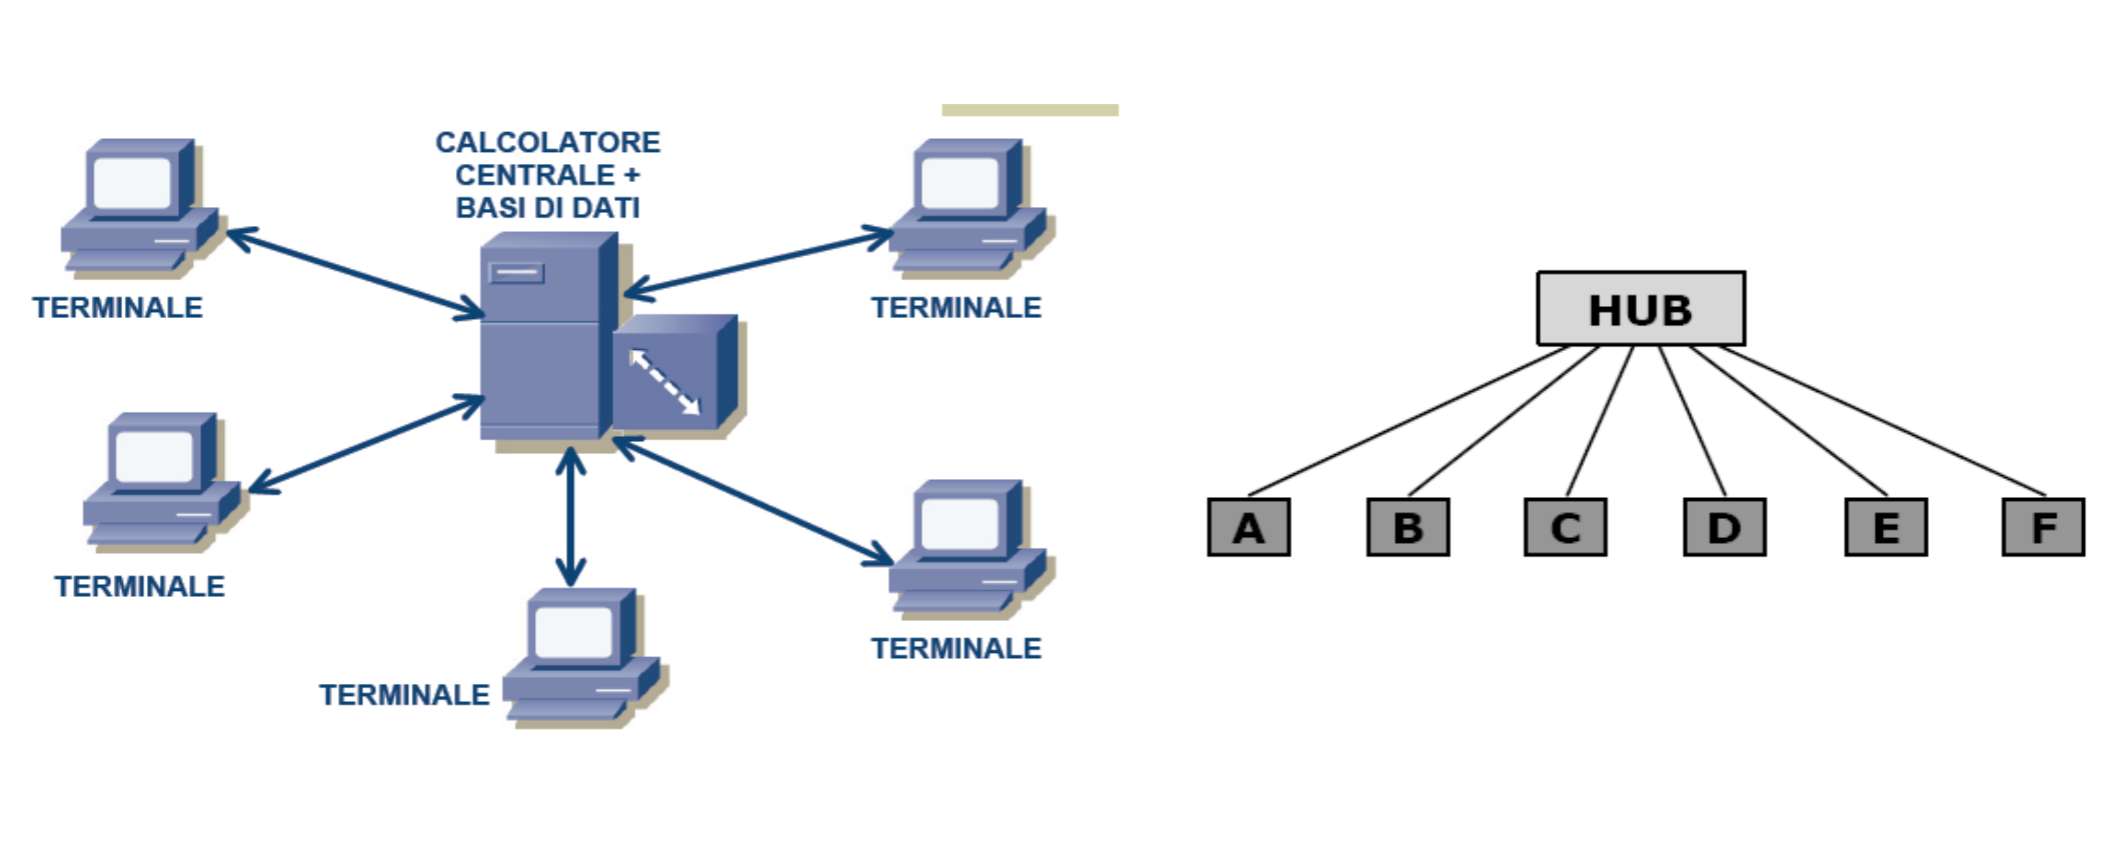
\includegraphics[width=1\textwidth]{Images/centralizzata.png}
    \end{figure}
\end{itemize}

\subsection{Standard}
La comunicazione tra nodi differenti e, possibilmente, basati su piattaforme hardware e/o software eterogenee necessita di \textcolor{red}{standard}.
Storicamente si parla di standard di un produttore: scambio di informazioni possibile solo per sistemi della stessa marca (sistemi \textcolor{red}{chiudi}).
Sono arrivati poi degli standard definiti da enti internazionali (livello di transizione dati).
\\ Il vantaggio è che assicurano un vasto mercato per i dispositivi e il software. Inoltre consentono a prodotti provenienti da fornitori \textcolor{red}{differenti} di comunicare.
\\ Di contro però è una tecnologia congelata e poi posono esserci più standard per la stessa funzione.
\pagebreak
\subsubsection{Standard ISO-OSI}
Lo standard ISO ha adottato un modello a strati. Il sistema di comunicazione viene diviso a strati ciascuno dei quali esegue una funzione predefinita.
Strati ISO/OSI possono essere separati in due categorie
\begin{itemize}
    \item funzioni dipendenti dalla rete (\textbf{Media layers});
    \item funzioni orientate all'applicazione (\textbf{Host layers}).
\end{itemize}
La funzione di ogni strato è codificata in una serie di regole e convenzioni usate per comunicare con lo strato remoto corrispondente (\textbf{protocollo}). 
Ogni strato fornisce dei servizi allo strato immediatamente superiore e utilizza inoltre dei servizi forniti dallo strato immediatamente inferiore.

\subsection{Protocollo}
La comunicazione tra entità richiede \textcolor{red}{cooperazione}, ossia collaborazione per il conseguimento di uno scopo comune. Le comunicazioni sono regolate tramite \textcolor{red}{protocolli}.
\\ \textbf{Protocollo}: insieme delle regole e convenzioni seguite da entità, dislocate su nodi distinti , che intendono comunicare per svolgere un compito comune. Tali regole hanno l'obiettivo di assicurare la cooperazione \textcolor{red}{efficiente} ed \textcolor{red}{affidabile}
per la comunicazione tra nodi.
\\ \textbf{Sintassi}: insieme e struttura dei comandi e delle risposte, formato dei messaggi.
\\ \textbf{Semantica}: significato dei comandi, delle azioni, delle risposte da effettuare al momento della trasmissione e ricezione dei messaggi.
\\ \textbf{Temporizzazione}: specifica delle possibilo sequenze temporali di emissione dei comandi e dei messaggi, nonchè eventuali risposte.
\\ Ciascun protoccolo ha un'interfaccia "interna" verso il livello superiore o inferiore, e un'interfaccia "esterna" verso il livello equivalente di un altro modo. 
\begin{figure}[H]
    \centering
    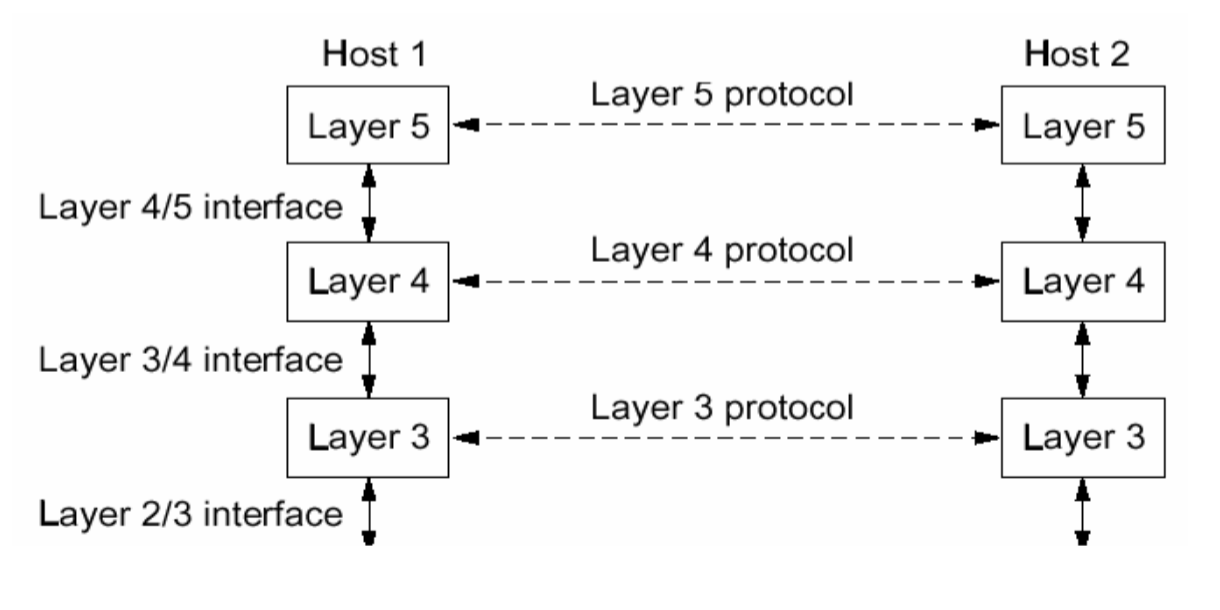
\includegraphics[width=0.5\textwidth]{Images/protocollo.png}
\end{figure}
\begin{itemize}
    \item \textbf{Service interface}("interna"):operazioni e servizi offerti al protocollo superiore.
    \item \textbf{Peer-to-peer interface}("esterna"): messaggi scambiati con un livello equivalente (peer) sull'altro nodo.
\end{itemize}
\begin{figure}[H]
    \centering
    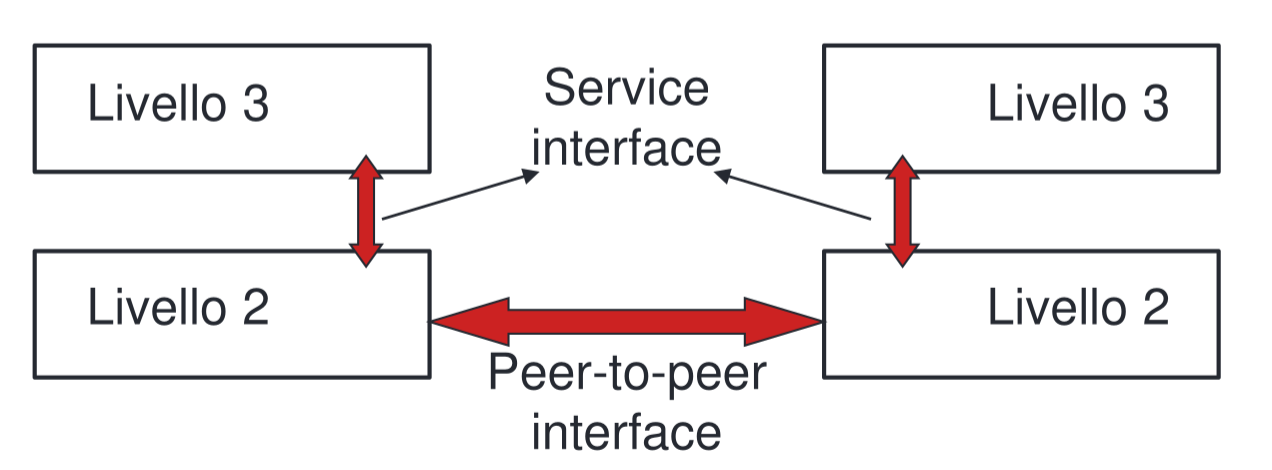
\includegraphics[width=0.5\textwidth]{Images/protocollo2.png}
\end{figure}
\begin{itemize}
    \item Comunicazione logica tra \textit{peer entity} (entità dello stesso livello).
\end{itemize}
\begin{figure}[H]
    \centering
    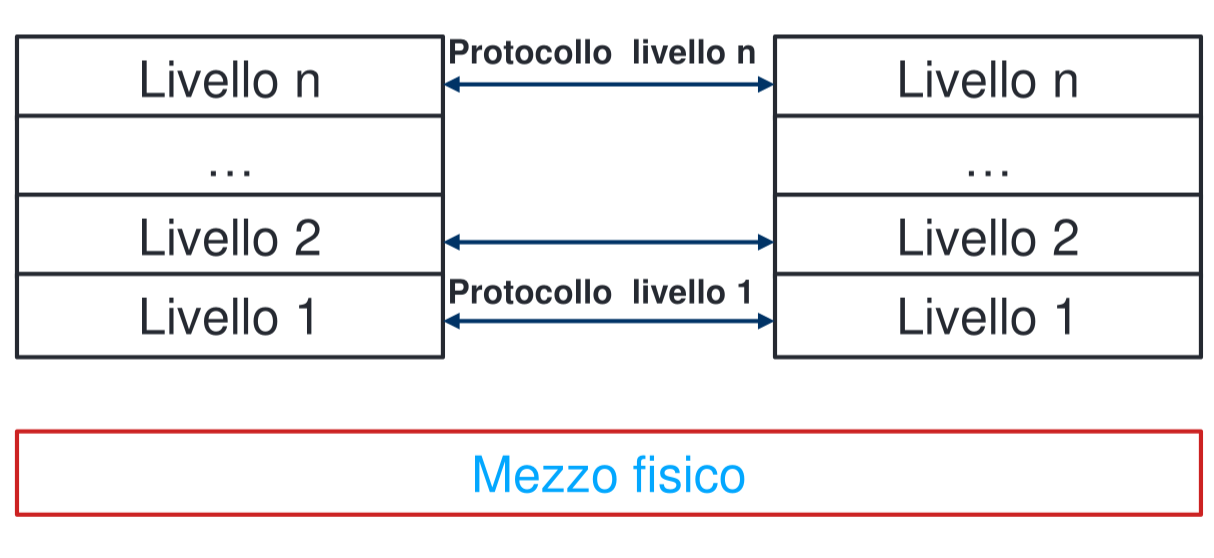
\includegraphics[width=1\textwidth]{Images/protocollo3.png}
\end{figure}
\begin{itemize}
    \item Comunicazione fisica (indiretta): la comunicazione tra \textit{peer entity} è diretta solo a livello hardware.
    \begin{figure}[H]
        \centering
        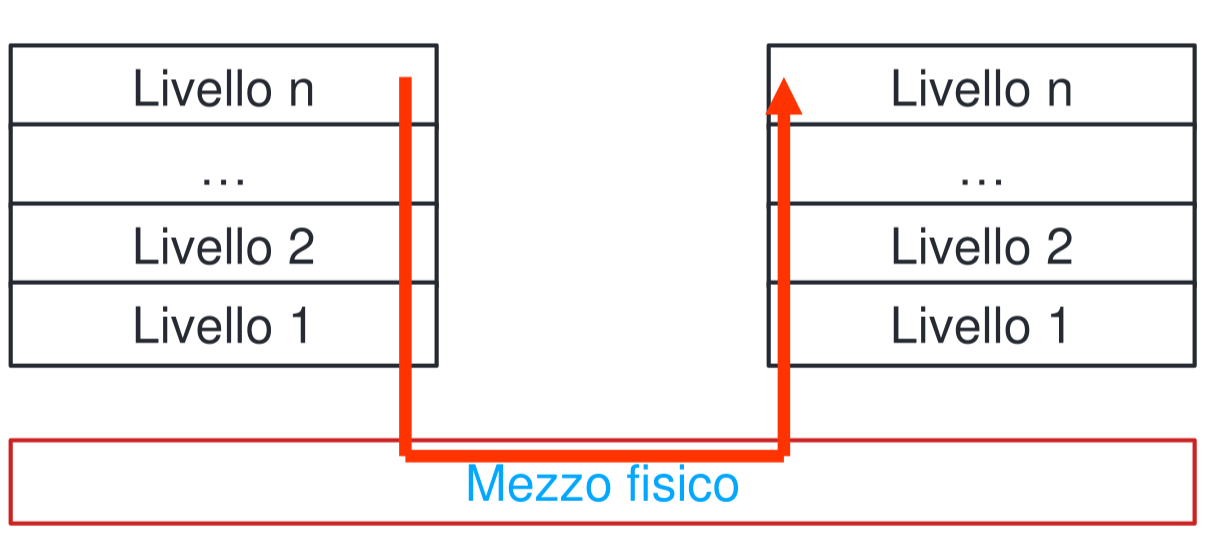
\includegraphics[width=0.5\textwidth]{Images/protocollo4.png}
    \end{figure}
\end{itemize}
Un messaggio si compone di:
\begin{itemize}
    \item \textbf{Header}: Protocol Control Information (PCI);
    \item \textbf{Dati}: Service Data Unit (SDU).
\end{itemize}
L'insieme delle due è chiamata \textbf{PDU} (Protocol Data Unit).
\begin{figure}[H]
    \centering
    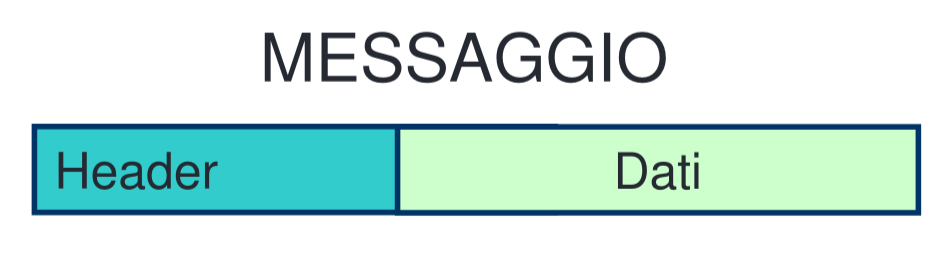
\includegraphics[width=0.5\textwidth]{Images/protocollo5.png}
\end{figure}
Incapsulamento del messaggio
\begin{figure}[H]
    \centering
    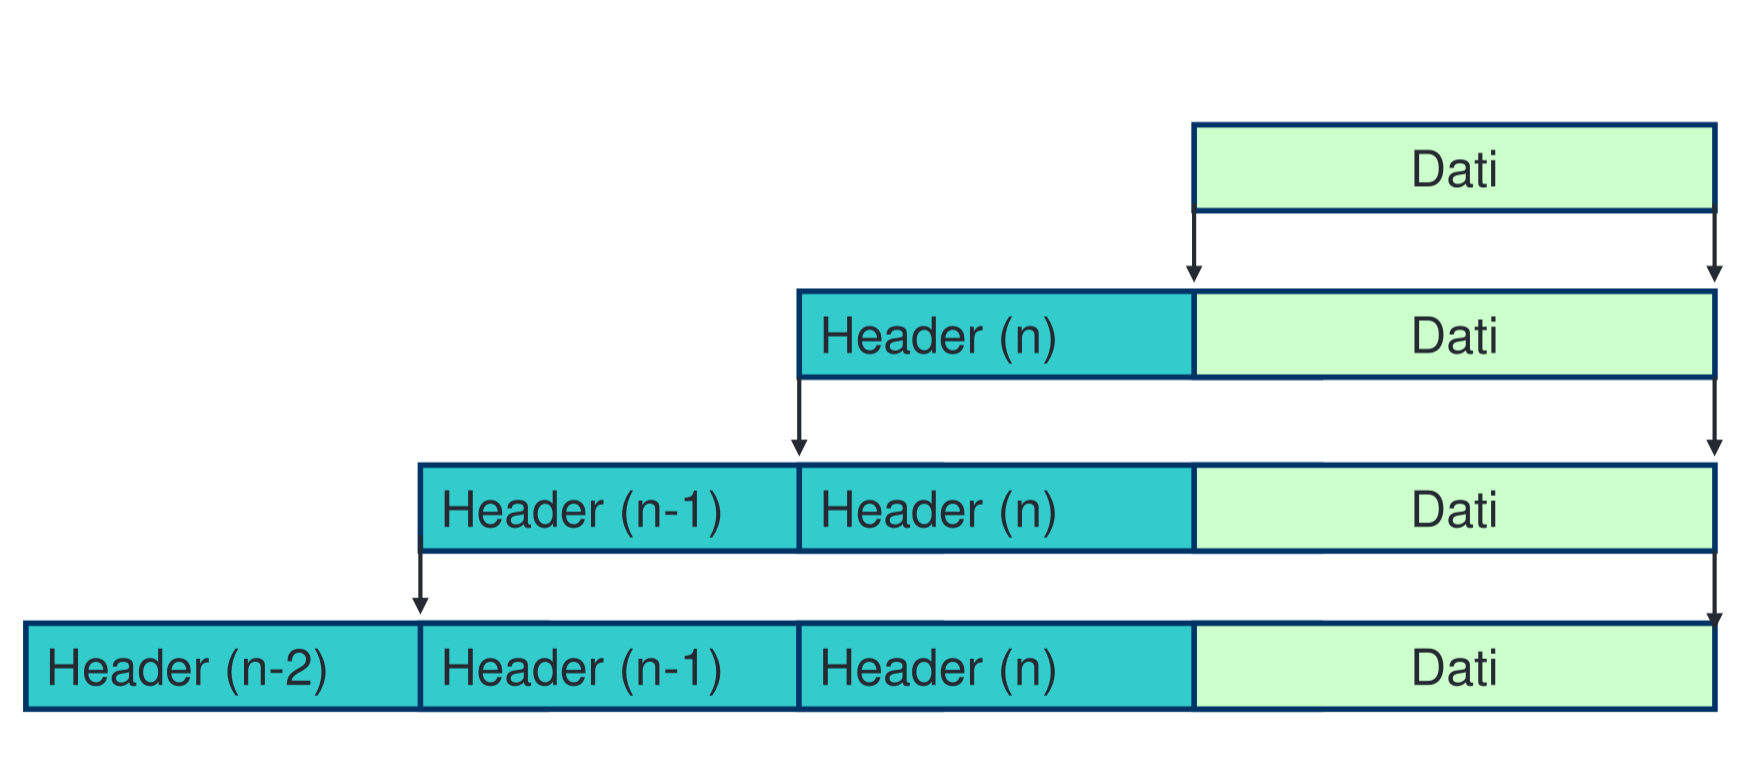
\includegraphics[width=0.5\textwidth]{Images/protocollo6.png}
\end{figure}
La comunicazione avviene \textbf{logicamente} tra \textit{peer}, ma in realtà attraversa tutti i livelli sottostanti, mediante \textbf{incapsulemnto del messaggio} a ciasun livello.
Il sistema di comunicazione richiede un insieme di protocolli tra loro cooperanti (detti \textbf{protocol suite} o \textbf{protocol stack}).

\section{HTML}
\subsection{Linguaggio di markup}
Linguaggio di markup modellato per rendere esplicita una particolare interpretazione di un testo. Con il markup per sistemi informatici, specifichiamo le modalità esatte di utilizzo del testo nel sistema stesso.
I linguaggi di markup sono i linguaggi più opportuni per strutturare e marcare i documenti in maniera indipendente dall'applicazione, favorendo la riusabilità, la flessibilità e la apertura ad applicazioni complesse.
\subsection{HyperText Markup Language}
HTML è un linguaggio per la creazione di pagine Web.
\begin{itemize}
    \item Standard per la rappresentazione.
    \item Descrive la struttura della pagina.
    \item Non è un linguaggio di programmazione, ma di markup.
    \item Descrive dati e regole su come mostrarli.
    \item Poche e semplici parole sintattiche.
\end{itemize}
\subsection{Browser}
È un programma per la navigazione Web. Richiede risorse attraverso il web (all'indirizzo richiesto) e la mostra nella finestra. Legge e inerpreta i documenti HTML, CSS, JavaScript, immagini sulla base di specifiche e standard.
\\ Un Browser è formato da:
\begin{itemize}
    \item \textbf{Layout Engine}: riceve input dal browser (URL bar, search box, mouse clicks and key presses) e li passa al \textcolor{red}{rendering engine}.
    \item \textbf{Rendering Engine}: riceve il codice HTML e lo interpreta visualizzandolo a video.
    \item \textbf{User interface}: controlli del browser, ad esempio, bottoni per andare avanti o indietro.
    \item \textbf{JavaScript engine}: engine che si prende cura di parsare ed eseguire codice JavaScript per poi ritornare il risultato dell'esecuzione.
    \item \textbf{Network Layer}: gestisce funzioni di rete, ad esempio, criptazione, richieste http, e tutte le configurazioni di rete.
    \item \textbf{Storage}: porzione di memoria dove il browser memorizza cached file, cookie, oggetti e dati create con JavaScript.
    \item \textbf{Operating System Interface}: componente che interagisce con il sistema operativo per disegnare diversi elementi e per gestire la finestra.
\end{itemize}
\begin{figure}[H]
    \centering
    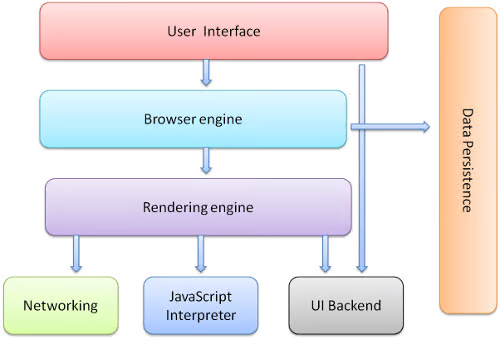
\includegraphics[width=0.5\textwidth]{Images/browser.png}
\end{figure}
\pagebreak
Il browser contiene anche tool per gli sviluppatori:
\begin{itemize}
    \item Debug pagina.
    \item Analisi stili e sorgenti dei file.
    \item Visualizzazione HTTP request e response.
    \item Accesso a cookie e storage.
    \item Etc..
\end{itemize}
\subsection{Struttura della pagina HTML}
\subsubsection{Tag}
I tag sono marcatori che identificano porzioni di testo. Permettono la personalizzazione della pagina, e di identificare e processare le porzioni di testo contrassegnate da una certa marcatura.
\\ Nome tag = nome funzione.
\\ Il tag ha la seguente struttura
\begin{center}
\texttt{<tag attributi>contenuto</tag>}
\end{center}
\subsection{Struttura della pagina}
Una pagina è formata da:
\begin{itemize}
    \item \textbf{Riga di intestazione}: \texttt{<!DOCTYPE HTML PUBLIC "-//W3C//DTD HTML 4.01
Transitional//IT">}. Indichiamo le specifiche W3C adottate. Esso dice al browser quale linguaggio è stato usato per il rendering.
    \item Il tag \textbf{\texttt{<html>}}: indica l'inizio di una pagina HTML. Tutto ciò compreso all'interno del tag \texttt{html} è il codice HTML.   
\begin{lstlisting}[language=HTML]
<html>
    ...
</html>
\end{lstlisting}
\item Documento HTML diviso in due:
\begin{itemize}
    \item Testa
    \item Corpo
\end{itemize}
\end{itemize}

\subsubsection{Testa}
La testa contiene informazioni non immediate. Descrive come il documento deve essere letto e interpretato. Contiene \textcolor{red}{meta-tag}, \textcolor{red}{script}, \textcolor{red}{stili}.
\\ È racchiuso nel tag \texttt{\textbf{<head>}}.
\subsubsection{Corpo}
Il corpo contiene il documento vero e proprio. Contiene tutti i tag per la realizzazione del sito Web. 
\\ È raachiuso nel tag \texttt{\textbf{<body>}}.
\subsection{Identazione}
Una buona norma è utilizzare caratteri di tabulazione. Aumenta la leggibilità, diminuendo così i tempi di modifica.
\subsection{Annidamento} 
Una caratteristica di HTML sono i \textcolor{red}{tag annidati}.
\subsection{Commenti}
I commenti aumentano la leggibilità del codice. Una buona norma è commentare \textbf{solo} le parti significative. Permettono di orientarsi meglio all'interno del codice.
\begin{lstlisting}[style=htmlstyle]
<!-- commento -->
\end{lstlisting}
\subsection{Maioscolo o minuscolo}
HTML è case unsensitive, mentre XHTML lo è. È consigliabile usare il carattere minuscolo.
\\ Inoltre non è sensibile anche agli spazi e alle linee vuote.
\subsection{Testa (\texttt{<head>})}
La testa contiene le informazioni/metadati relativi al documento. I browser di solito non presentano elementi che compaiono nella testa.
\subsubsection{Titolo}
L'elemento \texttt{<title>} permette di indicare il titolo della pagina. 
\subsubsection{Metadati}
L'elemento \texttt{<meta>} definisce le informazioni relative alla pagina piuttosto che contenuto vero e proprio. Contiene 3 attributi principali:
\begin{itemize}
    \item \textbf{Name}: contiene il nome della proprietà.
    \item \textbf{Content}: contiene il valore della proprietà.
    \item \textbf{http-equiv}: specifica le caratteristiche dell'HTTP responde header.
\end{itemize}
\begin{lstlisting}[style=htmlstyle]
<META NAME="author" CONTENT="Federico">
\end{lstlisting}
\subsubsection{Meta Tag - Keywords}
I meta tag indicano alcune informazioni sul contenuto del sito. Sono separate da virgole, punto e virgola e spazio.
Esse inoltre sono chiavi di ricerca. 
\\ Il motore di ricerca ricava le chiavi di indicizzazione. Bisogna fare attenzione nella scrittura delle keywords:
\begin{itemize}
    \item evitare termini generici e particolari;
    \item riportare termini italiani ed inglese;
    \item singolare e plurale.
\end{itemize}
Evitare di ripetere le stesse parole e usare Keyword astute.

\begin{lstlisting}[style=htmlstyle]
<meta name="keywords" content="calcio soccer tennis basket pallacanestro pallavolo volley inter milan juventus roma lazio...">
\end{lstlisting}
\subsubsection{Attributo HTTP-EQUIV}
Sono informazioni sulla comunicazione server-browser. Può essere utilizzato al posto dell'attributo name.
\\ L'attributo \texttt{http-equiv} fornisce un header HTTP per informazioni/valore dell'attributo content:
\begin{itemize}
    \item Può essere usato per simulare un HTTP response header.
    \item Gli HTTP server usano questo attributo per ottenere informazioni circa l'HTTP response header.
\end{itemize}
Alcuni valori sono: \texttt{content-type, default-style, refresh}
\\ Un esempio:
\begin{lstlisting}[style=htmlstyle]
<meta http-equiv="Content-Type" content="text/html; charset=iso-8859-1">
\end{lstlisting}
\subsection{Corpo (<body>)}
Il corpo di un documento contiene il contenuto vero e proprio. Il browser presenta il contenuto in diversi modi:
\begin{itemize}
    \item Browser visuali: è una tela su cui disegnare testi, immagini, colori, ... .
    \item Agenti audio: il contenuto stesso è parlato.
\end{itemize}
Esso contiene tutte le informazioni per la visualizzazione della pagina. Siccome gli style sheet sono il modo suggerito per specificare come verrà presentato un documento
gli attributi del \texttt{body} sono stati deprecati.
\subsection{Tag interni al body}
\subsubsection{Elementi inline vs block}
Alcuni elementi HTML nel body sono "\textcolor{red}{block-level}", altri "\textcolor{red}{inline}". Gli elementi block-level possono contenere elementi inline e altri elementi block-level, mentre gli elementi
inline contengono solo dati e altri elementi inline.
\subsubsection{Testo - Tag predefiniti}
I tag contenitori di testo sono block-level (ad eccezione di \texttt{<span>}).
\begin{itemize}
    \item \texttt{<h1>,<h2>, ...} - heading;
    \item \texttt{<p>} - paragrafo;
    \item \texttt{<span>} - elemento inline per raggruppare porzioni di testo (ad esempio per colorarlo in maniera diversa rispetto al resto);
    \item \texttt{<div>} - è un contenitore degli elementi HTML.
\end{itemize}
\paragraph{Titoli - Heading} \mbox{}\\
Sono previste sei grandezze predefinite per i titoli. Si va da \texttt{<h1>} che è la grandezza maggiore fino ad \texttt{<h6>} che è la grandezza minore.
\begin{lstlisting}[style=htmlstyle]
<h1>Titolo</h1>
\end{lstlisting}
\paragraph{Paragrafo} \mbox{}
Il paragrafo è l'unità base di suddivisione del testo.
\begin{lstlisting}[style=htmlstyle]
<p>Paragrafo</p>
\end{lstlisting}
\texttt{<p>} lascia una riga vuota prima e dopo il testo.
\paragraph{Blocco testo} \mbox{} \\
\texttt{<div>} è un blocco contenitore. Esso va a capo ma non lascia righe di spazio.
\begin{lstlisting}[style=htmlstyle]
<div>Blocco 1</div>
\end{lstlisting}
Non impone rappresentazioni di default. 
\paragraph{Contenitore} \mbox{} \\
È un contenitore generico e può essere annidato. È un elemento inline (continua sulla stessa riga del tag che lo contiene). Non va a capo.
\\ Non impone rappresentazioni di default (a parte il fatto di essere un elemento inline). 
\paragraph{Esempio} \mbox{}
\begin{lstlisting}[style=htmlstyle]
<h2>Titolo della pagina</h2>
<p>paragrafo 1</p>
<p>paragrafo 2</p>
<div>blocco 1</div>
<div>blocco 2
<span>contenitore 1</span>
<span>contenitore 2</span>
</div>
\end{lstlisting}
\subsubsection{Struttura della pagina con tag \texttt{<div>}}
\texttt{<div>} è uno tra i tag più utilizzati nella creazione di pagine Web, sopratutto nella creazione di layout. 
Esso fornisce un vero e proprio elemento strutturale della pagina.
Suddivide gli spazi in zone per progettare il sito in modo \textcolor{red}{semplice} e \textcolor{red}{dettagliato}.
\\ Molto utile quando usato insieme a fogli di stile.\\ 
\\ Facciamo un esempio: immaginando di dover costruire un sito, pensiamo a come esso debba essere strutturato, tipicamente abbiamo:
\begin{itemize}
    \item un contenitore (container);
    \item una parte alta (header);
    \item un corpo centrale (middle);
    \item un menù (navigation);
    \item una parte bassa (footer);
    \item spesso anche un pannello laterale (sidebar).
\end{itemize}
\begin{lstlisting}[style=htmlstyle]
<div id="container">
<div id="header">
<div id="navigation"></div><!--#navigation-->
</div><!--#header-->
<div id="main"></div><!--#main-->
<div id="sidebar"></div><!--#sidebar-->
<div id="footer"></div><!--#footer-->
</div><!--#container-->
\end{lstlisting}
\begin{figure}[H]
    \centering
    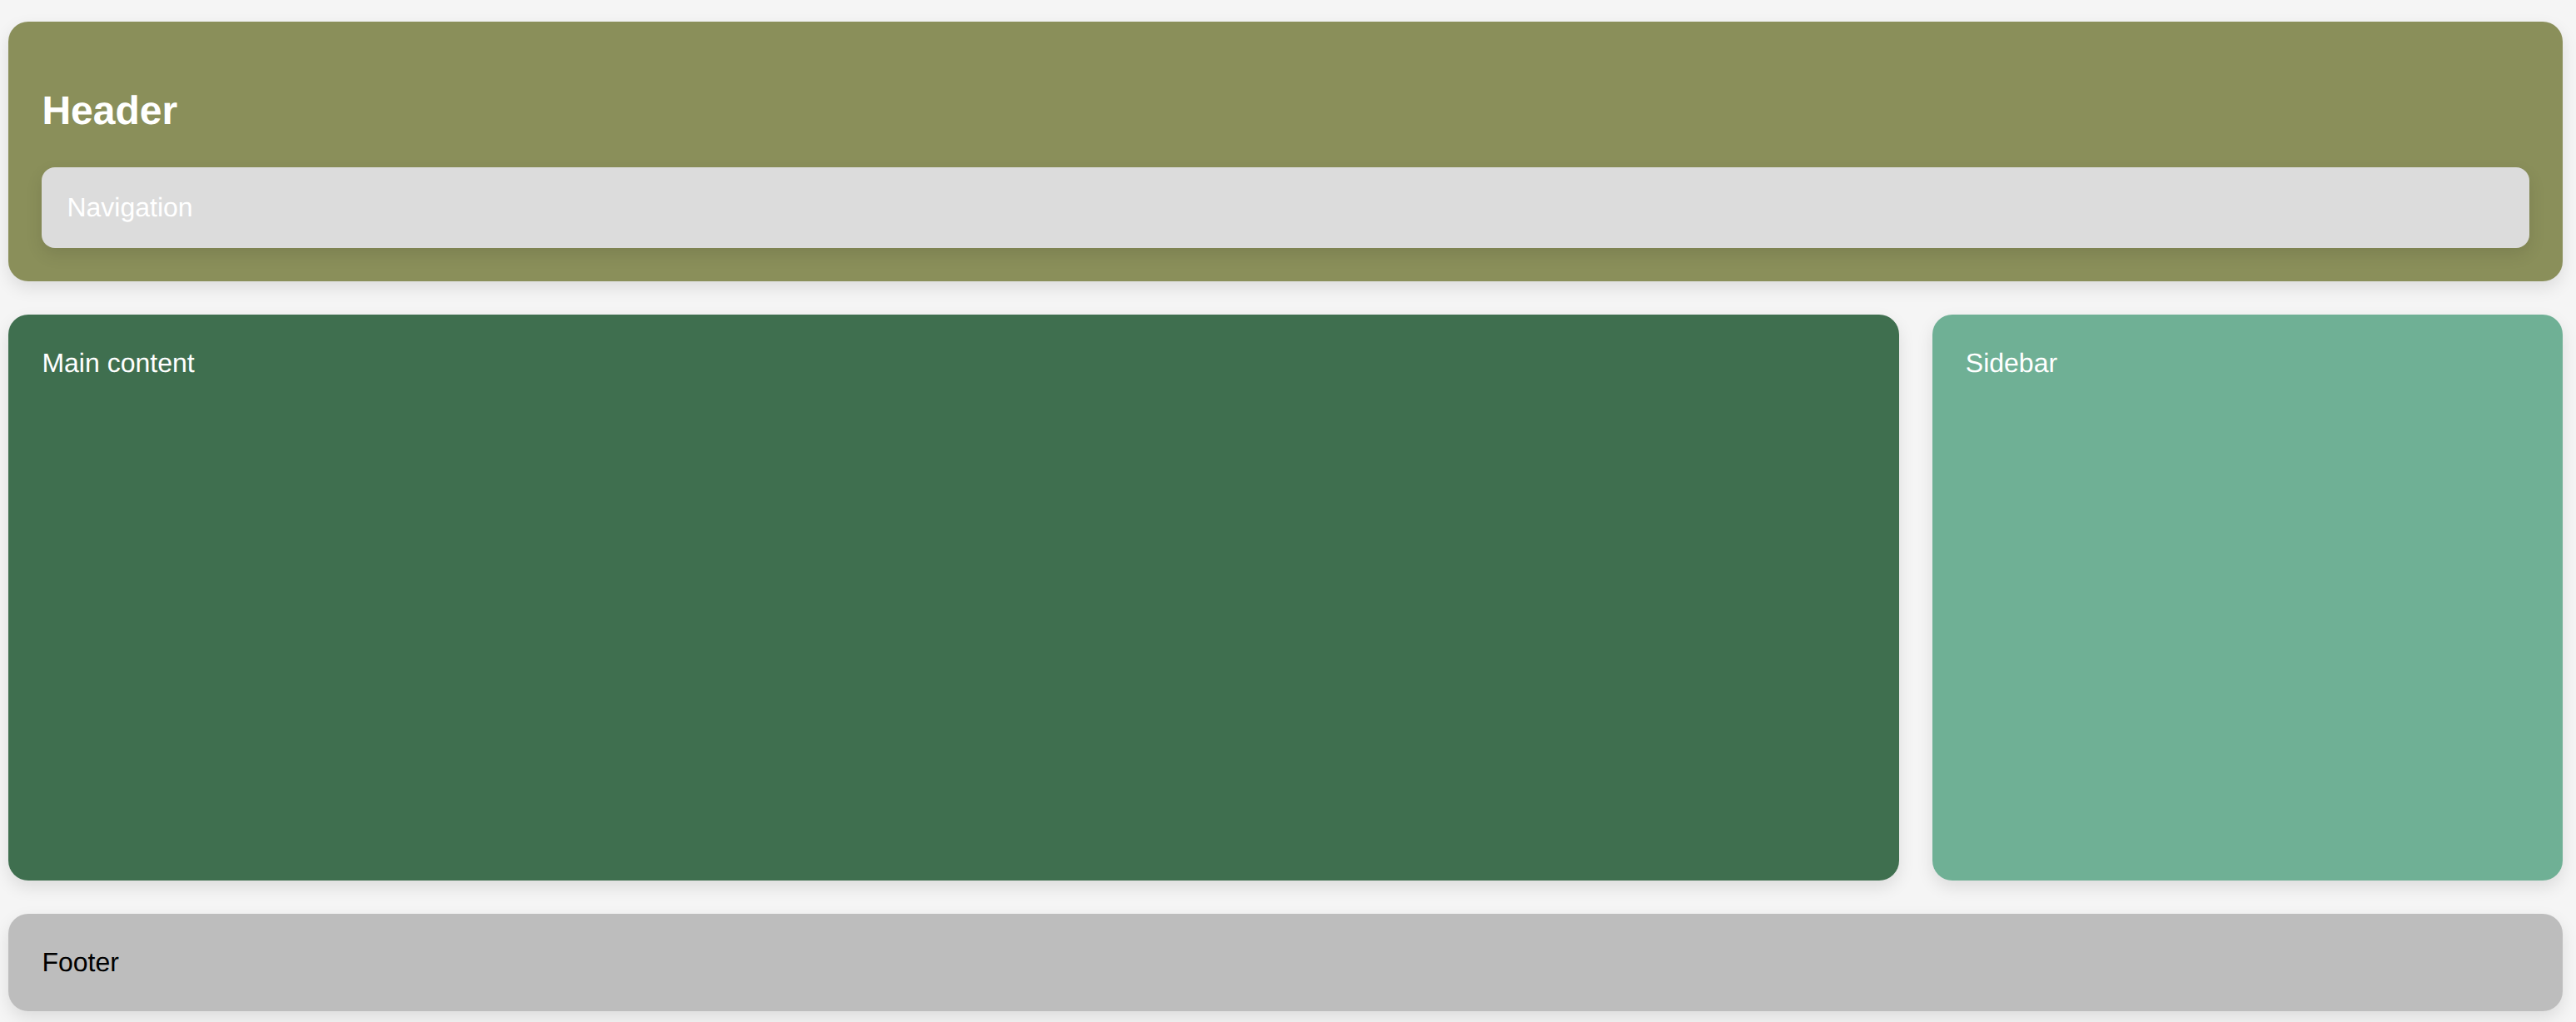
\includegraphics[width=1\textwidth]{Images/div.png}
\end{figure}
\pagebreak
\subsubsection{Testo - Stili}
Sono possibili due tipi di stili:
\begin{itemize}
    \item Fisici: definiscono lo stile grafico.
    \item Logici: forniscono informazioni sul ruolo svolto dal testo. Opzionalmente impongono uno stile grafico.
\end{itemize}
\paragraph{Stili fisici} \mbox{}
\begin{itemize}
    \item \texttt{<b>} bold: formatta il testo in \textbf{grassetto};
    \item \texttt{<i>} italic: formatta il testo in \textit{corsivo};
    \item \texttt{<u>} underline: \underline{sottolinea} il testo;
    \item \texttt{<strike>}: testo \sout{barrato} (usato per correzioni);
    \item \texttt{<sup>} apice: $E=mc^2$;
    \item \texttt{<sub>} pedice: $H_2O$.
\end{itemize}
\paragraph{Stili logici} \mbox{}
\begin{itemize}
    \item \texttt{<abbr>} abbreviazione: non comporta nessun cambiamento grafico;
    \item \texttt{<address>} indirizzo;
    \item \texttt{<cite>} citazioni: testo in corsivo;
    \item \texttt{<samp>} esempio: testo a spaziatura fissa.
\end{itemize}
\subsubsection{Testo - Font}
Il carattere predefinito è il \texttt{Times New Roman}. Esso però è poco leggibile. Meglio \texttt{Verdana}, \texttt{Arial} o \texttt{Helvetica}.
\begin{lstlisting}[style=htmlstyle]
<font face="verdana, arial, helvetica, sans-serif">testo</font>
\end{lstlisting}
È una buona norma utilizzare \textcolor{red}{caratteri sicuri} (sicuramente visualizzabili), non indicare un solo carattere e solo come ultima spiaggia sarà usato il \texttt{Times New Roman}.
\\ Per scegliere il colore del testo:
\begin{lstlisting}[style=htmlstyle]
<font color="#0000FF">testo blu</font>
\end{lstlisting}
LA scelta del colore e del carattere può essere fatta nello \textcolor{red}{stesso tag}.
\begin{lstlisting}[style=htmlstyle]
<font color="#0000FF" face="verdana">testo blu</font>
\end{lstlisting}
\paragraph{Font annidati} \mbox{}
\begin{lstlisting}[style=htmlstyle]
<font color="blue" face="verdana">
    testo blu
    <font color="red">
        testo rosso
    </font>
</font>
\end{lstlisting}
\paragraph{Dimensione del testo} \mbox{} \\
Si utilizza l'attributo \texttt{size} del tag \texttt{font}. Ci sono 2 modi per impostare la dimensione:
\begin{itemize}
    \item Valore tra 1 e 7.
    \begin{lstlisting}[language=html]
    <font size="3">Dimensione 3</font>
    \end{lstlisting}
    \item Valori relativi alla dimensione del font.
    \begin{lstlisting}[language=html]
    <font size="+2">Dimensione +2</font>
    \end{lstlisting}
    Utilizza la dimensione del font di base. Il tag \texttt{<basefont>} permette di cambiare il font di base.
\end{itemize}
\subsubsection{Elenchi}
Gli elenchi possono essere:
\begin{itemize}
    \item \textbf{ordinati};
    \item \textbf{non ordinati};
    \item \textbf{di definizioni}.
\end{itemize}
Sintassi:
\begin{lstlisting}[language=html]
<elenco>
    <elemento> primo elemento
    <elemento> secondo elemento
</elenco>
\end{lstlisting}
La chiusura dell'elemento è opzionale. La sintassi degli elenchi di definizione è leggermente diversa.
\paragraph{Elenchi ordinati} \mbox{} \\
Gli elementi sono numerati \textcolor{red}{progressivamente}.
\\ Il tag dell'elenco ordinato è \texttt{<ol>} (ordered list), mentre quello dell'elemento è \texttt{<li>} (list item).
\begin{lstlisting}[style=htmlstyle]
<div>Titolo</div>
<ol>
    <li>Primo elem prima tabella
    <li>Secondo elem prima tabella
    <ol>
        <li> Primo elem seconda tabella
        <li> Secondo elem seconda tabella
    </ol>
</ol>
\end{lstlisting}
\paragraph{Elenchi non ordinati} \mbox{} \\
Gli elementi non sono numerati. Si ottiene quindi un elenco puntato. Il tag è \texttt{ul} (unordered list).
\begin{lstlisting}[style=htmlstyle]
<ul>
    <li> Primo elemento
    <li> Secondo elemento
    <ul>
        <li> Primo elemento
        <li> Secondo elemento
    </ul>
</ul>
\end{lstlisting}
\paragraph{Elenco di definizioni} \mbox{}
\\ Per creare un elenco di definizione si utilizza il tag \texttt{dl} (definition list) e il termine da definire \texttt{<dt>} (definition term). Per la definizione del termine si utilizza il tag \texttt{<dd>} (definition description).
\begin{lstlisting}[style=htmlstyle]
<p> Titolo
<dl>
    <dt>&ltp&gt
        <dd>apertura paragrafo
    <dt>&ltdiv&gt
        <dd>apertura blocco di testo
    <dt>&ltspan&gt
        <dd>apertura elemento inline
    Altri tag...
</dl>
<dl>
\end{lstlisting}
\pagebreak
\subsection{Ipertestualità (Link)}
\subsubsection{Link}
I link sono formati da due componenti:
\begin{itemize}
    \item il contenuto (testo o immagine) che nasconde il collegamento;
    \item la risorsa puntata.
\end{itemize}
\begin{lstlisting}[style=htmlstyle]
<a href="indirizzo"> link </a>
\end{lstlisting}
La testa del link è \textit{link}, mente la coda è \textit{indirizzo}.
\\ La coda può essere una pagina HTML, un'immagine, documenti, altri file.
\subsubsection{Destinazioni}
Le destinazioni dei link possono essere:
\begin{itemize}
    \item Pagina HTML: aperta nel browser.
    \item Immagine (.gif, .jpeg): aperta nel browser.
    \item Altri documenti (.doc, .pdf):
    \begin{itemize}
        \item visualizzata nel browser;
        \item richiesta di salvataggio.
    \end{itemize}
    \item Altri file (.zip, .exe): richiesta di salvataggio.
\end{itemize}
\subsubsection{Caratteristiche dei link}
I link possono avere diversi stati:
\begin{itemize}
\item link a riposo: \textcolor[HTML]{0000FF}{blu};    
\item link visitato: \textcolor[HTML]{800080}{violetto};
    \item link attivo: passaggio da una pagina all'altra. Utile nel passato.
    \item link al passaggio del mouse: solo con fogli di stile.
\end{itemize}
\subsubsection{Manipolazione dei link}
\begin{itemize}
    \item \texttt{<body link="red">}: cambia il colore dei link;
    \item \texttt{<body vlink="green">}: cambia il colore dei link visited;
    \item \texttt{body alink="yellow">}: cambia il colore dei link attivi.
\end{itemize}
\subsubsection{Percorsi dei link}
I percorsi dei link possono essere:
\begin{itemize}
    \item \textcolor{red}{assoluti}: viene indicato il percorso per esteso;
    \item \textcolor{red}{relativi}: fanno riferimento alla posizione del file a cui si riferisce il link a partire dalla posizione della pagina che stiamo sviluppando.
\end{itemize}
\paragraph{Percorsi assoluti} \mbox{}
\begin{lstlisting}[style=htmlstyle]
<a href="http://www.miosito.it/cartella/miofile.html"> qui</a>
\end{lstlisting}
\paragraph{Percorsi relativi} \mbox{}
\begin{lstlisting}[style=htmlstyle]
<a href="sottodir/sottolink.html">Clicca qui</a>
\end{lstlisting}
\pagebreak
\subsubsection{Link interni o ancore}
Permette di creare un indice.
\begin{itemize}
    \item Ancora
    \begin{lstlisting}[style=htmlstyle]
    <a name="primo">ancora</a>
    \end{lstlisting}
    \item Riferimento all'ancora
    \begin{lstlisting}[style=htmlstyle]
    <a href="#primo"> vai all'ancora </a>
    \end{lstlisting}
    \item Riferimento ad inizio pagina
    \begin{lstlisting}[style=htmlstyle]
    <a href='#'>torna su</a>
    \end{lstlisting}
\end{itemize}
\subsubsection{Colorare i link}
Per colorare solo un link:
\begin{lstlisting}[style=htmlstyle]
<a href="...">
    <font color="green">
        link verde
    </font>
</a>
\end{lstlisting}
\subsubsection{Immagini}
Il web non è solo ipertesto, ma bensì ipermedia.
\begin{lstlisting}[style=htmlstyle]
<img src="pic.jpg" alt="description" width="128"height="128">
\end{lstlisting}
\begin{itemize}
    \item Attributo \texttt{src}: sorgente del file (percorso di memorizzazione file).
    \item Attributo \texttt{alt}: descrizione mostrata al passaggio sull'immagine.
    \item Attributi \texttt{width} e \texttt{height}: dimensioni dell'immagine.
\end{itemize}
Immagine come link:
\begin{lstlisting}[style=htmlstyle]
<a href="destinazione.html">
    <img src="pic.jpg">
</a>
\end{lstlisting}
\pagebreak
\subsection{Tabelle (table)}
Le tabelle si definiscono tramite l'elemento \texttt{<table>}. Ogni riga è definita con il tag \texttt{<tr>} contenuto in \texttt{table}.
Ogni cella è definita con il tag \texttt{<td>} contenuto in \texttt{<tr>}.
\\ Una riga può essere anche divisa in \textcolor{red}{table heading} usando l'elemento \texttt{<th>}. Di solito sono centrari e in grassetto.
\\ Elemento \texttt{<caption>} serve per definire la caption della tabella.
\begin{lstlisting}[style=htmlstyle]
<table style="width:100%">
    <tr>
        <td>Jill</td>
        <td>Smith</td>
        <td>50</td>
    </tr>
    <tr>
        <td>Eve</td>
        <td>Jackson</td>
        <td>94</td>
    </tr>
    <tr>
        <td>John</td>
        <td>Doe</td>
        <td>80</td>
    </tr>
</table>
\end{lstlisting}
\subsubsection{Bordi}
Per modificare i bordi della tabella si utilizza l'attributo \texttt{border}. Se non specificato nessun bordo:
\begin{lstlisting}[style=htmlstyle]
<table border="1" style="width:100%">
\end{lstlisting}
\subsubsection{Celle collassate in una riga/colonna}
Si utilizza l'attributo \texttt{rowsspan} per collassare un riga:
\begin{lstlisting}[style=htmlstyle]
<th rowspan="2">Telephone</th>
<td rowspan="2">Telephone</td>
\end{lstlisting}
Si utilizza l'attributo \texttt{colspan} per collassare una colonna:
\begin{lstlisting}[style=htmlstyle]
<th colspan="2">Telephone</th>
<td colspan="2">Telephone</td>
\end{lstlisting}
\pagebreak
\subsection{Form}
I form sono utilizzati per collezionare gli input degli utenti. È basato sull'elemento \texttt{<form>}. Esso specifica diversi elementi.
\subsubsection{Input}
È l'elemento più importante. Sono presenti diverse varianti a seconda da come si indica l'attributo \texttt{type}:
\begin{itemize}
    \item \texttt{text}: definisce input testo normale;
    \item \texttt{radio}: definisce un input radio button (per selezionare una tra diverse scelte);
    \item \texttt{submit}: definisce un bottone submit (per sottomettere il form).
\end{itemize}
\paragraph{Text input} \mbox{}\\
L'input text definisce un campo di testo di una linea. \texttt{<input type="password">} è un tipo speciale di campo testo dove il valore inserito viene nascosto.
\begin{lstlisting}[style=htmlstyle]
<form>
    First name:<br>
    <input type="text" name="firstname">
    <br>
    Last name:<br>
    <input type="text" name="lastname">
</form>
\end{lstlisting}
\paragraph{Text area} \mbox{} \\
Il text area definisce un campo testo a linee multiple.
\begin{lstlisting}[style=htmlstyle]
<textarea name="message" rows="10" cols="30">
    The cat was playing in the garden.
</textarea>
\end{lstlisting}

\paragraph{Radio button} \mbox{} \\
Il radio button definisce un input che permette \textbf{una} scelta tra diverse opzioni.
\begin{lstlisting}[style=htmlstyle]
<form>
    <input type="radio" name="sex" value="male" checked>Male
    <br>
    <input type="radio" name="sex" value="female">Female
</form>
\end{lstlisting}
\paragraph{Checkbox input} \mbox{} \\ 
La checkbox input definisce una serie di checkbox che permettono la scelta \textbf{multipla} tra diverse opzioni.
\begin{lstlisting}[style=htmlstyle]
<form>
    <input type="checkbox" name="vehicle1" value="Bike"> I have a bike
    <br>
    <input type="checkbox" name="vehicle2" value="Car"> I have a car
</form>
\end{lstlisting}
\paragraph{Drop-down list} \mbox{} \\
La drop down-drown list definisce un \textcolor{red}{menù a tendina}. L'elemento \texttt{<option>} definisce le possibili opzioni.
\begin{lstlisting}[style=htmlstyle]
<select name="cars">
    <option value="volvo">Volvo</option>
    <option value="saab">Saab</option>
    <option value="opel">Opel</option>
    <option value="audi">Audi</option>
</select>
\end{lstlisting}
\pagebreak
\paragraph{Submit button} \mbox{}\\
La submit button definisce un bottone per sottomettere la form ad un handler. L'handler è una pagina lato server che processa i dati del form. L'handler è definito con l'attributo \texttt{action}.
\begin{lstlisting}[style=htmlstyle]
<form action="action_page.php">
    First name:<br>
    <input type="text" name="firstname" value="Mickey">
    <br>
    Last name:<br>
    <input type="text" name="lastname" value="Mouse">
    <br><br>
    <input type="submit" value="Submit">
</form>
\end{lstlisting}
Permette anche di eseguire semplici azioni:
\begin{lstlisting}[style=htmlstyle]
<button type="button" onclick="alert('Hello World!')">Click Me!</button>
\end{lstlisting}
\subsubsection{Action attribute}
L'attributo \texttt{action} definisce le azioni che devono essere fatte quando il form è inviato.
La sottomissione viene comunque effettuata con il bottone submit. La pagina viene inviata a una pagina web lato server.
\\ Ad esempio uno script lato server gestisce la form inviata. Se l'attributo action è omesso, si considera la pagina corrente di default.
\subsubsection{Method attribute}
L'attributo \texttt{method} specifica l'operazione HTTP (GET o POST) da usare per inviare la form.
\\ GET, è l'opzione di default, viene usata per l'invio di form passive e \textcolor{red}{senza informazioni sensibili}. I dati inviati
sono visibili nell'\textcolor{red}{indirizzo}. È ottima per piccola quantità di dati.
\\GET è quindi utilizzata per l'invio di form che aggiornano dati, mentre POST fornisce maggiore sicurezza perchè i dati non sono visibili nell'indirizzo.
\subsubsection{Name attribute}
Ogni campo input deve avere un \textcolor{red}{nome}.
\begin{lstlisting}[style=htmlstyle]
<form action="action_page.php">
    First name:<br>
    <input type="text" name="firstname" value="Mickey">
    <br>
    Last name:<br>
    <input type="text" name="lastname" value="Mouse">
    <br><br>
    <input type="submit" value="Submit">
</form>
\end{lstlisting}
\subsubsection{Fieldset}
Per raggruppare campi di una form, si utilizza \texttt{<fieldset>}. Si può definire anche una caption per la form \texttt{<legend>}.
\begin{lstlisting}[style=htmlstyle]
<form action="action_page.php">
    <fieldset>
        <legend>Personal information:</legend>
        First name:<br>
        <input type="text" name="firstname" value="Mickey">
        <br>
        Last name:<br>
        <input type="text" name="lastname" value="Mouse">
        <br><br>
        <input type="submit" value="Submit">
    </fieldset>
</form>
\end{lstlisting}
\subsubsection{Altri attributi}
\begin{itemize}
    \item \texttt{value}: definisce il valore iniziale;
    \item \texttt{readonly}: specifica che il valore non può essere cambiato;
    \item \texttt{disabled}: specifica un campo disabilitato e non utilizzabile (non viene inviato);
    \item \texttt{size}: specifica la dimensione in caratteri del campo;
    \item \texttt{maxlength}: specifica la dimensione massima del contenuto del campo.
\end{itemize}
\pagebreak
\subsection{XHTML}
XHTML è quasi identito ad HTML, ma è più stringente. È supportato dai principali browser.
\paragraph{Perchè utilizzare XHTML} \mbox{}
\\ Molte pagine Web contengono HTML errato. Il seguente codice viene visualizzato bene nella maggior parte dei casi anche 
se non segue le regole di HTML:
\begin{lstlisting}[style=htmlstyle]
<html>
    <head>
        <title>This is bad HTML</title>
    </head>
    <body>
        <h1>Bad HTML</h1>
        <p>This is a paragraph</p>
    </body>
</html>
\end{lstlisting}
Diversi browser che eseguo su device diversi richiedono maggiori risorse o potenza coputazionale per interpretare un markup sbagliato.
\\ XHTML combina HTML e XML.
\section{Bootstrap}
\paragraph{Web design reattivo} \mbox{} \\
 Il responsive web design riguarda la creazione di siti web che si adattano automaticamente per avere un bell'aspetto su tutti i dispositivi, dai piccoli
telefoni ai desktop di grandi dimensioni. \\ Bootstrap è il framework HTML, CSS e JavaScript più popolare per lo sviluppo di siti Web responsive e mobile-first.
\paragraph{} Bootstrap è un framework front-end gratuito per uno sviluppo web più rapido e semplice. Bootstrap include modelli di progettazione basati su HTML e CSS per tipografia, moduli, pulsanti, tabelle, navigazione, modali, caroselli di immagini e molti altri, oltre al plug-in JavaScript opzionali.
\\ Bootstrap dà anche la possibilità di creare facilmente design reattivi.
\subsection{Come ottenere Bootstrap?}
Ci sono due modi per iniziare ad usare Bootstrap:
\begin{itemize}
    \item scaricare Bootstrap da \url{getbootstrap.com} e seguire le istruzioni da lì;
    \item includere Bootstrap da un CDN (Content Delivery Network).
\end{itemize}
\subsubsection{CDN di Bootstrap}
Bisogna includere i seguenti CSS, Javascript e jQuery di Bootstrap da MaxCDN nella pagina web:
\begin{lstlisting}[style=htmlstyle]
<!-- Ultimo CSS Bootstrap compilato e minimizzato -->
<link rel="stylesheet" href="https://maxcdn.bootstrapcdn.com/bootstrap/3.3.7/css/bootstrap.min.css">
\end{lstlisting}
\begin{lstlisting}[style=htmlstyle]
<!-- JavaScript Bootstrap piu recente compilato -->
<script src="https://maxcdn.bootstrapcdn.com/bootstrap/3.3.7/js/bootstrap.min.js"></script>
\end{lstlisting}
\begin{lstlisting}[style=htmlstyle]
<!-- ultima libreria jQuery -->
<script src="https://code.jquery.com/jquery-latest.js"></script>
\end{lstlisting}
Vantaggio dell'utilizzo di Bootstrap CDN: molti utenti hanno già scaricato Bootstrap da MaxCDN visitando un altro sito. Di conseguenza, verrà caricato dalla cache quando visitano il sito,
il che porta a tempi di caricamento più rapidi. Inoltre, la maggior parte dei CDN farà in modo che una volta che un utente richiede un file da esso, verrà servito dal server più vicino a loro,
il che porta anche a tempi di caricamento più rapidi.
\subsection{Creare una pagina Web con Bootstrap}
Bisogna aggiungere il doctype HTML5 siccome Bootstrap utilizza elementi HTML e proprietà CSS di questo doctype.
\begin{lstlisting}[style=htmlstyle]
<!doctype html>
<html lang="en">
    <head>
        <meta charset="utf-8">
        <meta name="viewport" content="width=device-width, initial-scale=1">
        <title>Bootstrap demo</title>
        <link href="https://cdn.jsdelivr.net/npm/bootstrap@5.3.3/dist/css/bootstrap.min.css" rel="stylesheet" integrity="sha384-
            QWTKZyjpPEjISv5WaRU9OFeRpok6YctnYmDr5pNlyT2bRjXh0JMhjY6hW+ALEwIH" crossorigin="anonymous">
    </head>
    <body>
        <h1>Hello, world!</h1>
        <script src="https://cdn.jsdelivr.net/npm/bootstrap@5.3.3/dist/js/bootstrap.bundle.min.js" integrity="sha384-
            YvpcrYf0tY3lHB60NNkmXc5s9fDVZLESaAA55NDzOxhy9GkcIdslK1eN7N6jIeHz" crossorigin="anonymous"></script>
    </body>
</html>
\end{lstlisting}
Bootstrap è un mobile-first:
\begin{itemize}
    \item Bootstrap 3 è progettato per rispondere ai dispositivi mobili. Gli stili mobile-first fanno parte del frameword principale.
    \item Per garantire un rendering e uno zoom al tocco corretti, bisogna aggiongere il tag \texttt{<meta>} all'interno dell'elemento \texttt{<head>}.
    \begin{lstlisting}[style=htmlstyle]
    <meta name="viewport" content="width=device-width, initial-scale=1">
    \end{lstlisting}
    \item La parte \texttt{width=device-width} imposta la larghezza della pagina in modo che segue la larghezza dello schermo del dispositivo (che varierà a seconda del dispositivo).
    \item La parte \texttt{initial-scale=1} imposta il livello di zoom iniziale quando la pgina viene caricata per la prima volta dal browser.
\end{itemize}
\paragraph{Contenitori} \mbox{} \\
Bootstrap richiede anche un elemento contenitore per racchiudere i contenuti del sito. Ci sono due classi di contenitori tra cui scegliere:
\begin{itemize}
    \item La classe \texttt{.container} fornisce un \textbf{contenitore a larghezza fissa reattivo}.
    \item La classe \texttt{.container-fluid} fornisce un \textbf{contenitore a larghezza intera}, che copre l'intera larghezza del viewport.
\end{itemize}
\begin{figure}[H]
    \centering
    
\includegraphics[width=1\textwidth]{Images/container.png}
\end{figure}
\textbf{Nota}: i contenitori non sono modificabili (non è possibile inserire un contenitore all'interno di un altro contenitore).
\pagebreak
\subsection{Griglie Bootstrap}
Il sistema a griglia di Bootstrap consente fino a 12 colonne nella pagina. Se non si desira utilizzare tutte e 12 le colonne singolarmente, si possono raggruppare insieme per creare colonne più larghe.
\begin{lstlisting}[style=htmlstyle]
<div class="col-md-12">Si estende su 12 colonne</div>
<div class="col-md-6">Intervallo 6</div><div class="col-md-6">Intervallo 6</div>
<div class="col-md-4">Intervallo 4</div><div class="col-md-8">Intervallo 8</div>
<div class="col-md-4">Intervallo 4</div><div class="col-md-4">Intervallo 4</div> <div class="col-
md-4">Intervallo 4 </div>
\end{lstlisting}
Il sistema a griglia di Bootstrap è reattivo e le colonne si riorganizzeranno automaticamente a seconda delle dimensioni dello schermo.
\\ È indivisuato quindi dalla classe \texttt{.col-(nome breakpont)-*}
\begin{figure}[H]
    \centering
    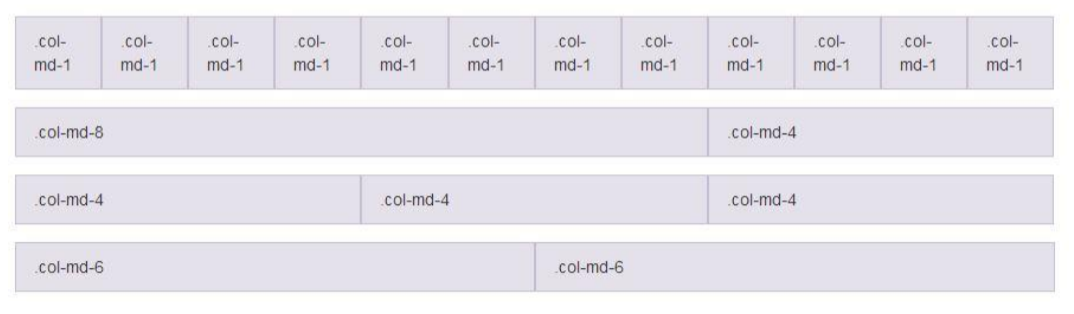
\includegraphics[width=1\textwidth]{Images/grid_system.png}
\end{figure}
È possibile innestare griglie nelle colonne creando delle \texttt{.row} nelle colonne, reiterando il meccanismo.
\begin{figure}[H]
    \centering
    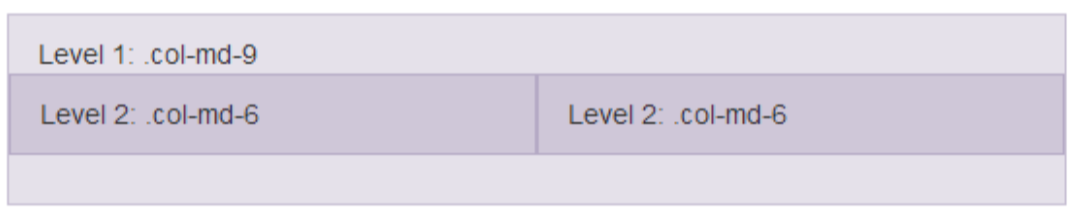
\includegraphics[width=1\textwidth]{Images/grid_system2.png}
\end{figure}
È possibile gestire i salti di colonna con gli offset \texttt{col-md-offset-*}.
\begin{figure}[H]
    \centering
    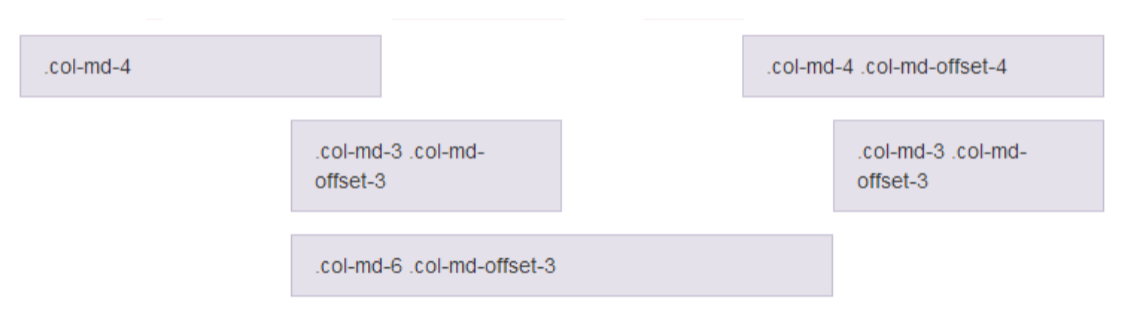
\includegraphics[width=1\textwidth]{Images/grid_system3.png}
\end{figure}
Di default è possibe gestire 5 dimensioni del viewport:
\begin{itemize}
    \item Extra small (\texttt{.col-xs-*}), per gli smartphone.
    \item Small (\texttt{.col-sm-*}), per i tablet.
    \item Medium (\texttt{.col-md-*}), per i desktop.
    \item Large (\texttt{.col-lg-*}), per i desktop larghi.
    \item Extra large (\texttt{.col-xl-*}), per i desktop molto larghi.
\end{itemize}
\subsection{Nuovo Flexbox grid system}
Con il nuovo Grid System non dobbiamo più indicare il numero nella classe della colonna, basterà usare solo la classe \texttt{.col-(nome breakpoint)} e si adatteranno in automatico allo spazio disponibile.
\begin{lstlisting}[style=htmlstyle]
<div class="row">
    <div class="col-xs"> 1 of 3 </div>
    <div class="col-xs"> 2 of 3 </div>
    <div class="col-xs"> 3 of 3 </div>
</div>
\end{lstlisting}
Possiamo allineare le righe in verticale:
\begin{figure}[H]
    \centering
    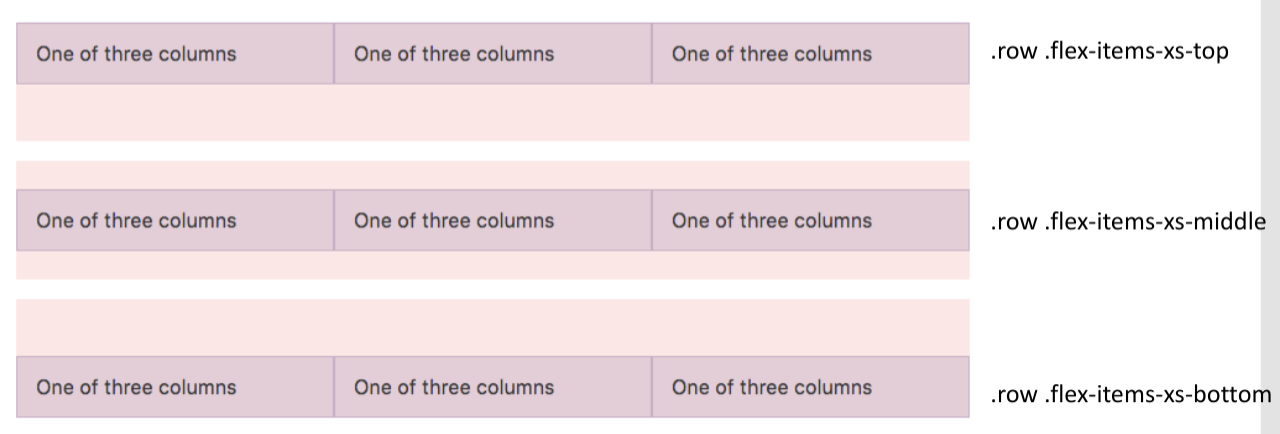
\includegraphics[width=1\textwidth]{Images/nuovo_flexbox.png}
\end{figure}
... e anche le colonne
\begin{figure}[H]
    \centering
    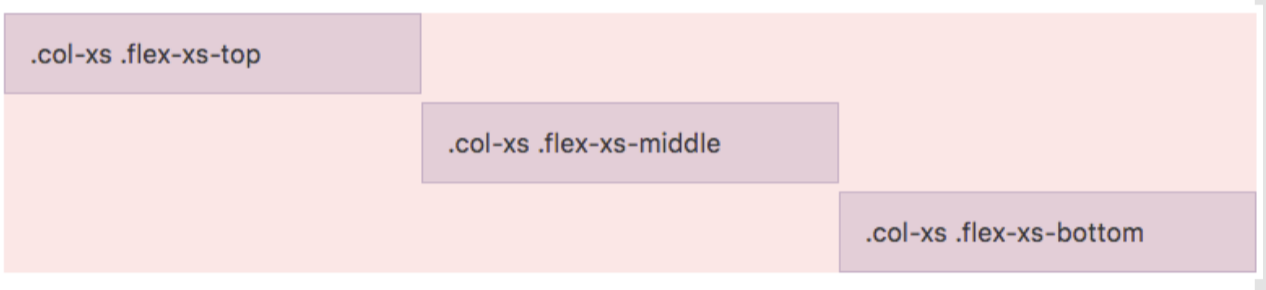
\includegraphics[width=1\textwidth]{Images/nuovo_flexbox2.png}
\end{figure}
Riordino orizzontale
\begin{figure}[H]
    \centering
    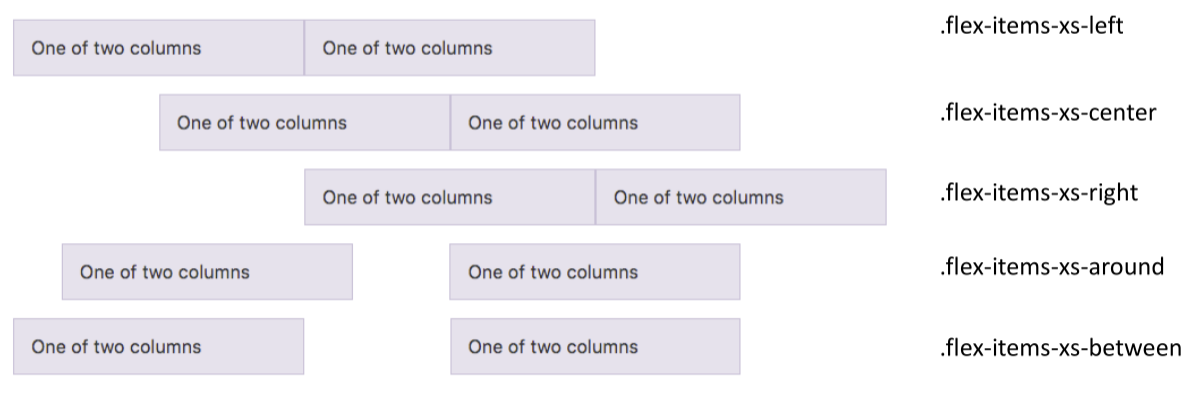
\includegraphics[width=1\textwidth]{Images/nuovo_flexbox3.png}
\end{figure}
Riordino della posizione
\begin{figure}[H]
    \centering
    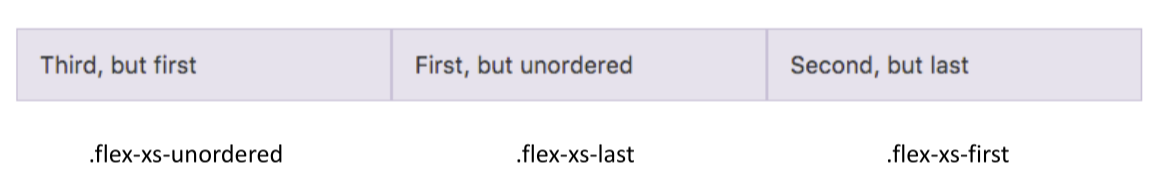
\includegraphics[width=1\textwidth]{Images/nuovo_flexbox4.png}
\end{figure}
\subsection{Classi di griglia}
Il sistema di griglia di Bootstrap ha quattro classi:
\begin{itemize}
    \item xs;
    \item sm;
    \item md;
    \item lg.
\end{itemize}
Le classi di cui sopra possono essere combinate per creare layout più dinamici e flessibili.
\subsubsection{Struttura di base di una griglia Bootstrap}
\begin{lstlisting}[style=htmlstyle]
<div class="row">
    <div class="col-*-*"></div>
</div>
<div class="row">
    <div class="col-*-*"></ div>
    <div class="col-*-*"></div>
    <div class="col-*-*"></div>
</div>
<div class="row">
...
< /div>
\end{lstlisting}
Primo; creare una riga (\texttt{<div class="row"}). Quindi, aggiungere il numero desiderato di colonne (tag con classi \texttt{.col-*-*} appropriate). Nota che in numeri in \texttt{.col-*-*} dovrebbero sempre sommare fino a 12 per ogni riga.
\subsection{Tabelle Bootstrap}
Un tavolo Bootstrap di base ha una \textbf{leggera imbottitura e solo divisori orizzontali}. La classe \texttt{.table} aggiunge uno stile di base a una tabella:
\begin{itemize}
    \item \textbf{righe a strisce}: la classe \texttt{.table-striped} aggiunge strisce zebrate a una tabella.
    \item \textbf{Tavolo bordato}: la classe \texttt{.table-bordered} aggiunge bordi su tutti i lati della tabella e delle celle.
    \item \textbf{Righe al passaggio del mouse}: la classe \texttt{.table-hover} abilita uno stato hover sulle righe della tabella.
    \item \textbf{Tabelle reattive}: la classe \texttt{.table-responsibe} crea una tabella reattiva. La tabella scorrerà quindi orizzontalmente su dispositivi di piccole dimensioni (768 px). Quando si visualizza su qualcosa di più largo di 768 px, non c'è differenza.
\end{itemize}
\subsection{Immagini Bootstrap}
\begin{itemize}
    \item \textbf{Angoli arrotondati}: la classe \texttt{.img-rounded} aggiunge angoli arrotondati a un'immagine.
    \item \textbf{Cerchio}: la classe \texttt{.img-circle} modella l'immagine in un cerchio.
    \item \textbf{Miniatura}: la classe \texttt{.img-thumbnail} modella l'immagine in una miniatura.
    \item \textbf{Immagine reattive}: le immagini sono disponibili in tutte le dimensioni. Così fanno gli schermi. Le immagini reattive si adattano automaticamente alle dimensioni dello schermo. Crea immagine reattive aggiungendo una classe \texttt{.img-responsive} al tag \texttt{<img>}. L'immagine verrà quindi ridimensionata in modo corretto rispetto all'elemento genitore. La classe \texttt{.img-responsive} applica \texttt{display: block}; e larghezza massima: 100\%: e altezza: \texttt{auto}; all'immagine.
\end{itemize}
\subsection{Bottoni Bootstrap}
Stili dei pulsanti: Bootstrap fornisce 7 stili di pulsanti con le seguenti classi:
\begin{itemize}
    \item \texttt{.btn-predefinito};
    \item \texttt{.btn-primary};
    \item \texttt{.btn-success};
    \item \texttt{.btn-info};
    \item \texttt{.btn-warning};
    \item \texttt{.btn-danger};
    \item \texttt{.btn-link}.
\end{itemize}
\subsubsection{Elementi del pulsante Bootstrap}
Le classi di pulsanti possono essere utilizzaate sui seguenti elementi:
\begin{itemize}
    \item \texttt{<a>};
    \item \texttt{<pulsante>};
    \item \texttt{<input>}.
\end{itemize}
\subsubsection{Dimensioni dei pulsanti}
Bootstrap fornisce quattro dimensioni di pulante con le seguenti classi:
\begin{itemize}
    \item \texttt{.btn-lg};
    \item \texttt{.btn-md} (dimensione predefinita);
    \item \texttt{.btn-sm};
    \item \texttt{.btn-xs}.
\end{itemize}
\subsubsection{Pulsanti a livello di blocco}
Un pulsante a livello di blocco copre l'\textbf{intera larghezza} dell'elemento genitore. Per fare ciò si aggiunge la classe \texttt{.btn-block}. 
\subsubsection{Pulsanti attivi/disabilitati}
Un pulsante può essere impsotato su uno stato attivo (appare premuto) o disabilitato (non cliccabile): la classe \texttt{.active} fa apparire premuto un pulsante e la classe \texttt{.disabled} rende un pulsante non cliccabile.
\subsection{Personalizzazione}
Il codice sorgente di Bootstrap può essere personalizzato:
\begin{itemize}
    \item Attraverso un tool online (V3).
    \item Less (V3).
    \item Sass (V3 e V4).
\end{itemize}
\subsection{Cards}
Wells, thumbnails e panels ci lasciano in favore delle cards.
\subsection{Nuovi helpers}
Nuovi classi di supporto per gestire margin, padding e proprietà display
\begin{itemize}
    \item \texttt{.pb-0} (padding-bottom: 0;);
    \item \texttt{-p-3} (padding: 3rem;);
    \item \texttt{mt-0} (margin-top: 0;);
    \item \texttt{.ml-1} (margin-left: 1rem;);
    \item \texttt{.mx-auto} (margin-left: auto; margin-right: auto;);
\end{itemize}
Migliorate le classi di supporto per allineare il testo in base al breakpoint:
\begin{itemize}
    \item \texttt{text-xs-left} (-right, -center);
    \item \texttt{text-sm-left} (-right, -center);
    \item \texttt{text-md-left} (-right, -center);
    \item \texttt{text-lg-left} (-right, -center);
    \item \texttt{text-xl-left} (-right, -center);
\end{itemize}
Migliorate le classi di supporto per allineare gli elementi in base al breakpoint:
\begin{itemize}
    \item .float-xs-left (-right);
    \item .float-sm-left (-right);
    \item .float-md-left (-right);
    \item .float-lg-left (-right);
    \item .float-xl-left (-right);
\end{itemize}
Migliorate le classi per nascondere o mostrare elementi in base al breakpoint: \texttt{.hidden-xs} diventa \texttt{.hidden-xs-up}.
\\ Ad esempio: \texttt{.hidden-md-up} nasconderà tutti gli elementi dal breakpoint md in su.
\subsection{Introduzione a SASS}
\textbf{SASS}: è un \textbf{pre-processore CSS}, un meta-linguaggio che ci permette di usare una sintassi più simile a quella dei linguaggi di programmazione offrendo moltissimi vantaggi tra cui una \textbf{maggiore manutenibilità del codice}.
SASS è nato per rimediare a disordine e ripetizioni, per introdurre una strututra formale dei CSS, migliorare la scrittura del codice e renderlo più manutenibile e ottimizzare la gestione delle media queries e andare incontro alle esigenze del mercato in crescita di dispositivi mobili.
\subsubsection{Come funziona}
\begin{figure}[H]
    \centering
    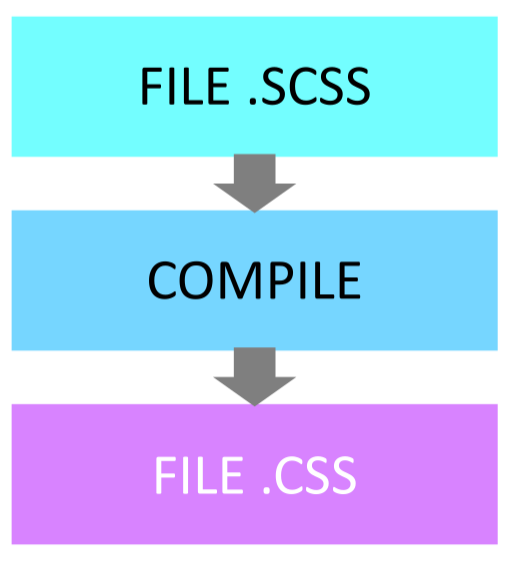
\includegraphics[width=0.25\textwidth]{Images/sass.png}
\end{figure}
\pagebreak
\subsubsection{Caratteristiche di Sass}
\begin{itemize}
    \item \textbf{Nesting}: possibilità di nidificare i selettori ottenendo un codice pulito.
    \item \textbf{Variabili}: come in altri linguaggi è un insieme di dati modificabili istuati in una porzione di memoria;
    \item \textbf{Importazione}: permette di importare altri file \texttt{scss} o \texttt{css} senza generare un grosso numero di richieste HTTP che rallenterebbero inevitabilmente il sito.
    \item \textbf{Funzioni}: in Sass esistono dei set di funzioni preconfezionate per effettuare diverse operazioni, è inoltre possibile sviluppare funzioni personalizzate;
    \item \textbf{Mixin}: permette di realizzare dei set riutilizzabili di regole CSS;
    \item \textbf{Logica condizionale}: @if, @else, @else if.
    \item \textbf{Cicli}: @for, @each, @while.
    \item \textbf{Compass, scount, ecc...}: framework opensource che offrono un'ampia gamma di mixin, funzioni e variabili preconfezionati.
\end{itemize}
\subsubsection{Nesting}
Con il \textbf{nesting} basta dichiarare una sola volta il nome dell'elemento radice per inestare le altre regole figlie all'interno.
\begin{figure}[H]
    \centering
    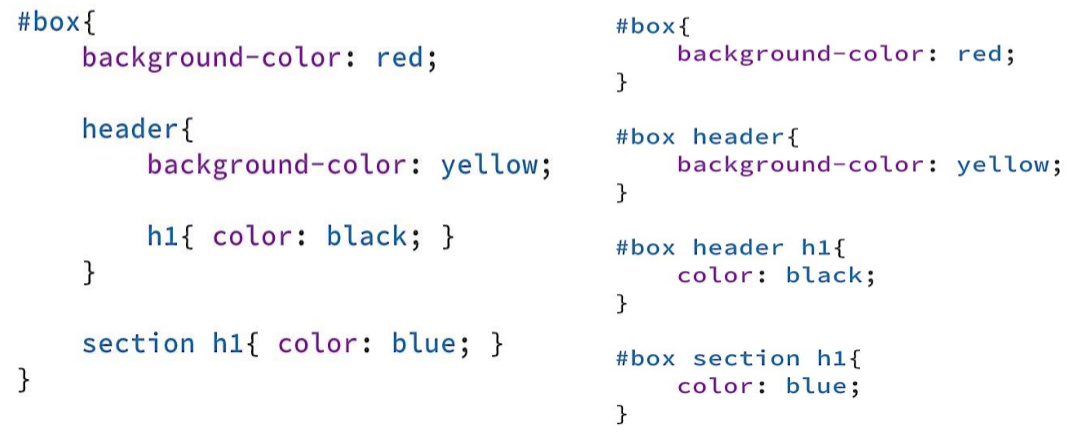
\includegraphics[width=0.75\textwidth]{Images/nesting.png}
\end{figure}
\textbf{SASS} fornisce il selettore speciale "\textbf{\&}" che, utilizzato all'interno di un \textbf{nesting} farà riferimento all'elemento radice.
\begin{figure}[H]
    \centering
    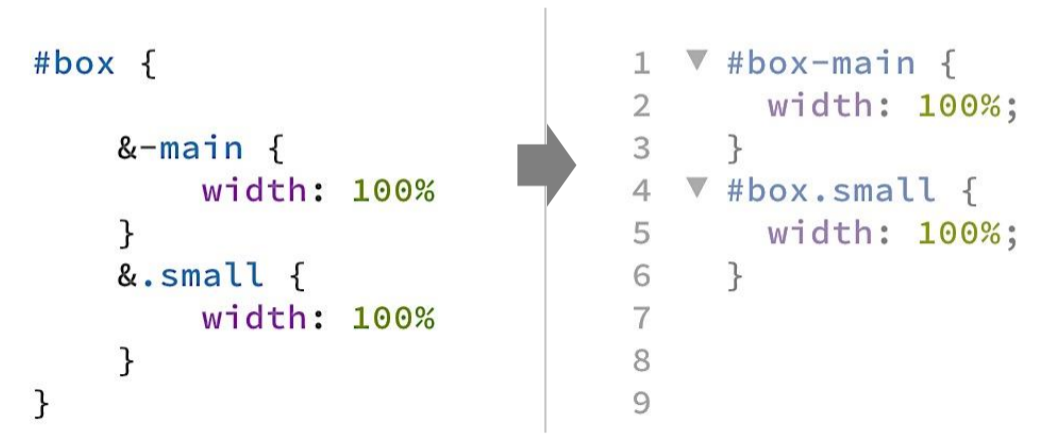
\includegraphics[width=0.75\textwidth]{Images/nesting2.png}
\end{figure}
\pagebreak
"\textbf{\&}" può essere utilizzato per definire le pseudoclassi di un elemento.
 \begin{figure}[H]
     \centering
     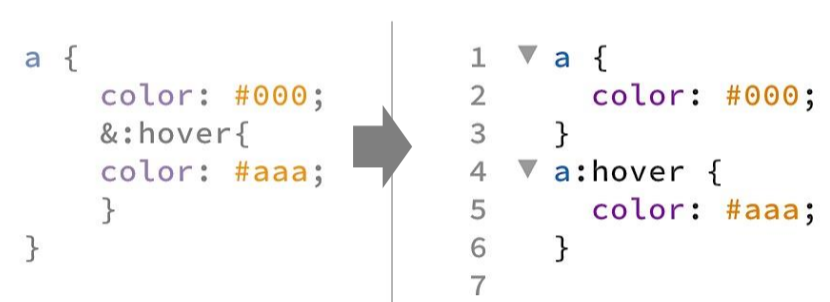
\includegraphics[width=0.75\textwidth]{Images/nesting3.png}
 \end{figure}
\subsubsection{Variabili}
\textbf{Variabili}: come nei linguaggi di programmazione il concetto di variabile è pressoché identico, una variabile \textbf{SASS} è un contenitore virtuale di:
\begin{itemize}
    \item stringhe di testo;
    \item valori numerici;
    \item numeri in virgola mobile;
    \item valori booleani.
\end{itemize}
Ad esempio possiamo creare dei set di colori:
\begin{figure}[H]
    \centering
    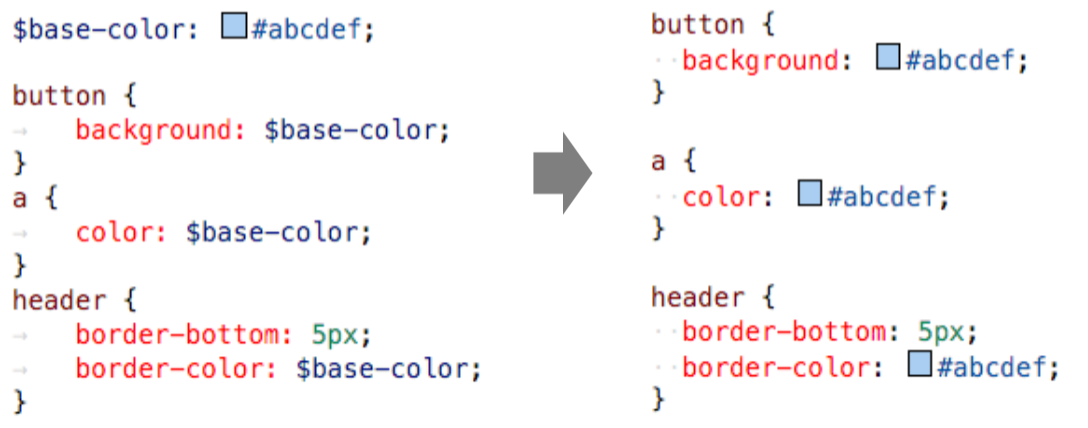
\includegraphics[width=0.75\textwidth]{Images/colori.png}
\end{figure}
Oppure gestire facilmente le media queries.
\subsection{Appunti utili}
\begin{itemize}
    \item Se voglio fare in modo che un testo sia colorato di un certo colore, utilizzare la classe \texttt{.text-white}.
    \item Per dare un spazio tra un elemento e l'altro, utilizzare le classi di \textbf{spacing}.
    \item Al posto di \texttt{<small>} si può usare la classe \texttt{.small}.
    \item Utilizzare \texttt{<span>} per raggruppare un testo e applicare uno stile specifico.
    \item Per cambiare il colore si può usare anche la classe \texttt{.text-*colore*}. Aggiungedoci -*valore* si aggiunge la trasparenza.
    \item Per modificare font testo, utilizzare \texttt{.fw-fold}, ad esempio.
    \item Per creare un testo con la sidebar, utilizzare \texttt{overflow-auto}.
    \item Per far sì che una immagine entri correttamente in un contenitore, utilizzare la proprietà CSS \texttt{object-fit: cover;}.
\end{itemize}
\pagebreak
\section{JavaScript}
\subsection{Introduzione}
\subsubsection{Applicazioni Web}
Le risorse in rete identificata tramite URL è di 3 tipi:
\begin{itemize}
    \item pagina \textbf{statica} (HTML) il cui contenuto è \textbf{fisso}, definito nel momento in cui la pagina è stata scritta;
    \item pagina \textbf{dinamica} il cui contenuto viene generato (selezionato, composto) al momento della richiesta (o della visualizzazione);
    \item \textbf{applicazione web}: software sviluppato e utilizzato attraverso attraverso tecnologie web;
    \begin{itemize}
        \item linguaggi di mark-up, scripting e programmazione;
        \item teconologie client-side e server-side;
    \end{itemize}
\end{itemize}
\subsubsection{Applicazioni web: linguaggi}
\begin{itemize}
    \item linguaggi di mark-up descrivono documenti strutturati (contenuto + struttura).
    \item linguaggi di programmazione descrivono programmi come sequenza di istruzioni;
    \item linguaggi di scripting, tipo particoalre di linguaggio di programmazione, per scrivere script.
\end{itemize}

\subsubsection{Applicazioni web: linguaggi di programmazione e scripting}
Un programma è un insieme di istruzioni, mentre i linguaggi di programmazione sono linguaggi per scrivere programmi. Un linguaggio è composto da:
\begin{itemize}
    \item \textbf{Alfabeto}: insieme di simboli con cui si possono costruire i termini del linguaggio (lessico).
    \item \textbf{Sintassi}: definita da una grammatica che fornisce regole di composizione dei termini in frasi bene formate del linguaggio.
    \item \textbf{Semantica}: definisce il significato delle frasi ben formate del linguaggio.
\end{itemize}
Un \textbf{analizzazatore sintattico} (parser) analizza frasi e decide se sono frasi ben formate del linguaggi o no.
\\ Lingiaggio di programmazione: 
\begin{itemize}
    \item lessico: "keywords" del linguaggio;
    \item frasi ben formate: istruzioni (programmi);
    \item semantica: esecuzione del programma.
\end{itemize}
Il programmatore scrive il programma sorgente utilizzando un linguaggio ad "alto livello". Occore però tradurre il programma sorgente in un programma composto da istruzioni
in un linguaggio macchina (programma eseguibile). Le tecniche per effettuare questa traduzione sono:
\begin{itemize}
    \item \textbf{Compilazione}: traduzione effettuata da strumenti chiamati compilatori.
    \item \textbf{Interpretatori}: traduzione effettuata da strumenti chiamati interpreti.
    \item \textbf{Approccio misto}.
\end{itemize}
La traduzione effettuata dal compilatore è specifica per una data macchina. Inoltre genera un \textcolor{red}{file eseguibile} (.exe). Il vantaggio è che è efficiente. Lo svantaggio è che è poco flessibile.
\\ La traduzione effettuata dall'interprete interpreta un programma (traduzione simultanea). Ogni istruzione viene tradotta in un insieme di istruzioni nel linguaggio macchina della piattaforma specifica ed eseguita. C'è un interprete specifico per ogni piattaforma. Il vantaggio è che è flessibile, di contro però è poco efficiente.
\\ Nell'approccio misto, il programma sorgente viene tradotto in formato intermedio (bytecode) indipendente dalla macchina (compilatore). Il programma in formato intermedio verrà poi interpretato dall'interprete.
\\ L'approccio misto somma i vantaggi dei due approcci. È efficiente e flessibile. 
\pagebreak
\subsubsection{Applicazioni Web}
Pagine web "dinamiche": il contenuto viene generato al momento della richiesta/visualizzazione. Si basano su linguaggi di programmazione e scripting:
\begin{itemize}
    \item tecnologie client-side (pagine "debolmente" dinamiche): 
    \begin{itemize}
        \item elaborazione lato client (browser);
        \item scripting client-side (JavaScript), Java Applet, Adobe Flash.
    \end{itemize}
    \item tecnologie server-side (pagine "fortemente" dinamiche): \begin{itemize}
        \item elaborazione lato server (web server);
        \item scripting server-side (PHP, Active Server Pages, Java Server Page), programmi (Java Servlet), Ruby, Python, Perl, (Javascript).
    \end{itemize}
\end{itemize}
Le applicazioni web si sviluppano su 3 livelli logici:
\begin{itemize}
    \item Presentazione - HTML, CSS.
    \item Intermedio - JavaServlet, JSP, PHP, ASP, JavaScript, Flash.
    \item Dati - RDBMS, XML, JSON.
\end{itemize}
Client-side:
\begin{figure}[H]
    \centering
    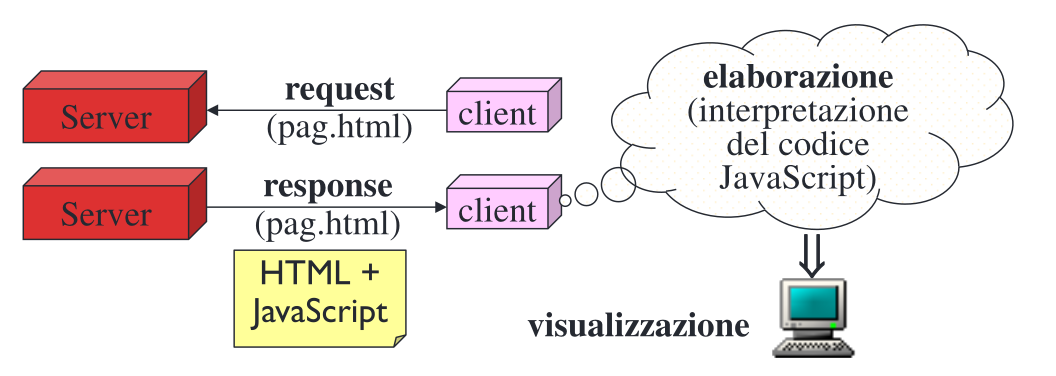
\includegraphics[width=0.5\textwidth]{Images/client_side.png}
\end{figure}
Server-side:
\begin{figure}[H]
    \centering
    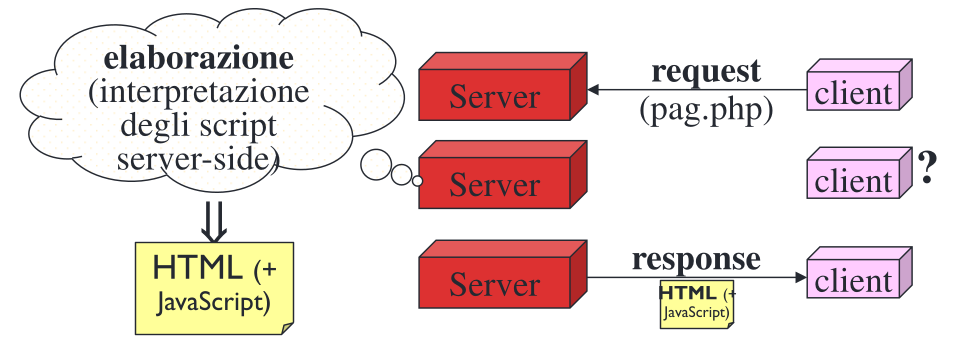
\includegraphics[width=0.5\textwidth]{Images/server_side.png}
\end{figure}
\subsubsection{Architettura server-side}
\begin{figure}[H]
    \centering
    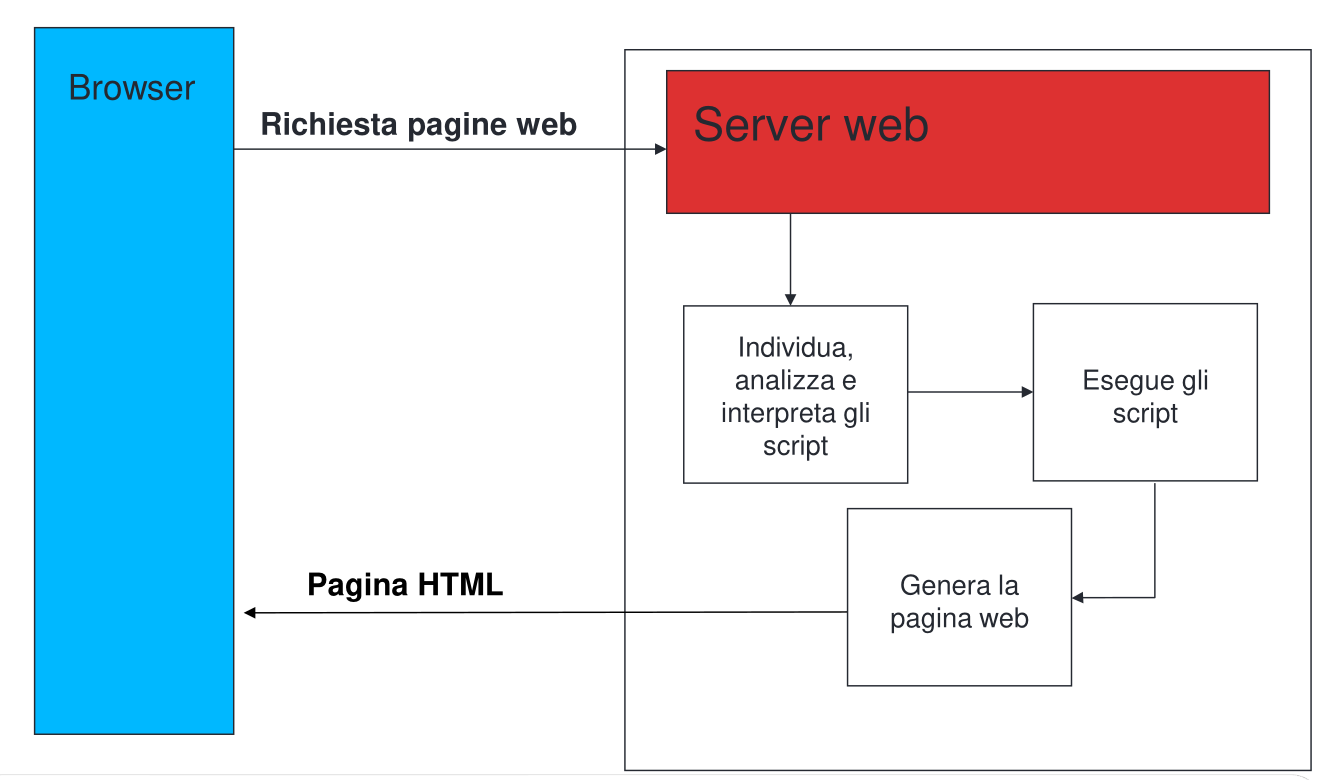
\includegraphics[width=0.5\textwidth]{Images/arch_server_side.png}
\end{figure}
\pagebreak
\subsubsection{Architettura client-side}
\begin{figure}[H]
    \centering
    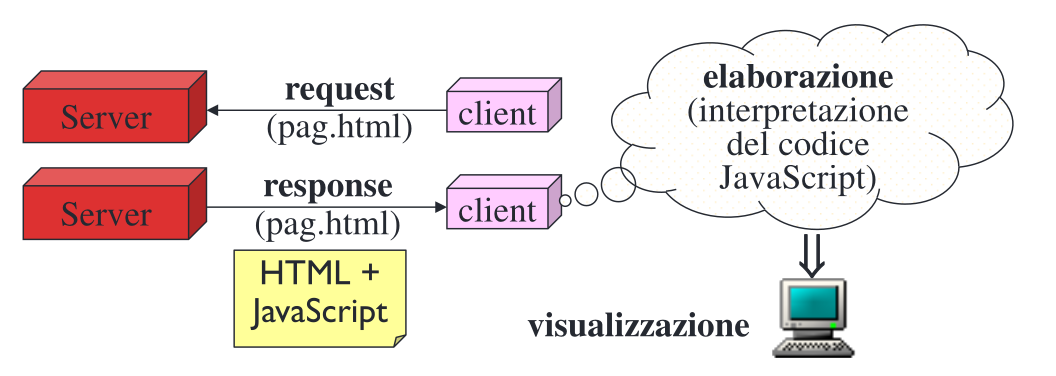
\includegraphics[width=1\textwidth]{Images/client_side.png}
\end{figure}
Per visualizzare una pagina Web "debolmente" dinamica NON HO bisogno di un server: posso aprire la pagina fornendo al browser il path sul file system locale.
\\ Per visualizzare una pagine Web autenticamente dinamica H(che utilizza una tecnologia server-side) HO bisogno di un server: devo connettermi al server (e richiedere la pagina) tramite un URL.
\\ Se chiedo al browser di visualizzare il codice sorgente della pagina:
\begin{itemize}
    \item Nel caso di una pagina Web "debolmente" dinamica vedo l'HTML + il codice "dinamico" client-side.
    \item Nel caso di una pagina Web autenticamente dinamica vedo solo l'HTML: al posto del codice "dinamico" server-side, il server ha infatti sostituito il risultato dell'alaborazione (cioè codice HTML).
\end{itemize}
Esistono degli approcci ibridi, utilizzando sia tecnologie client-side che teconologie server-side. Un esempio è AJAX e JQuery.
\subsubsection{AJAX}
\begin{figure}[H]
    \centering
    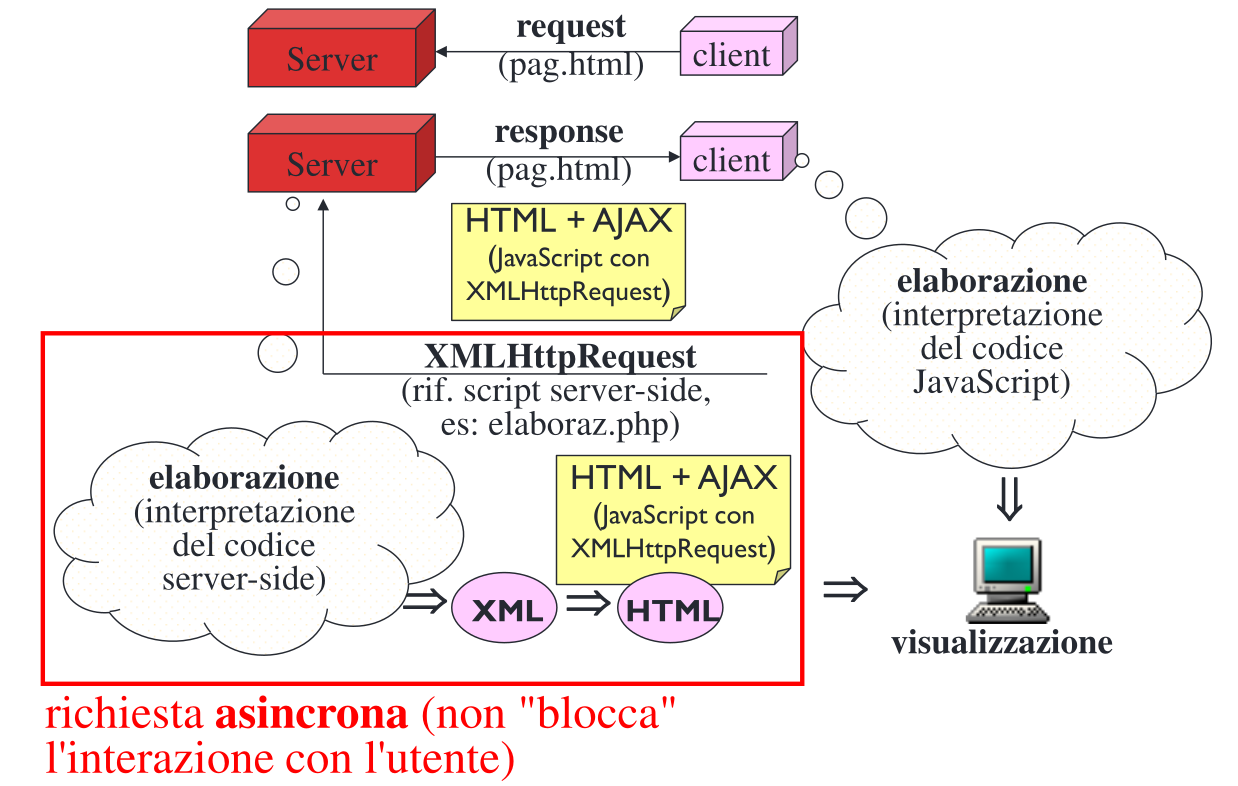
\includegraphics[width=0.5\textwidth]{Images/ajax}
\end{figure}
\pagebreak
\subsection{JavaScript}
JavaScript è un linguaggio di scripting, tipicamente utilizzato client-side. Nonostante la somiglianza nel nome, è un linguaggio completamente distinto da Java. Come tutti i linguaggi di scripting, è interpretato: il sorgente non deve essere compilato per essere eseguito.
L'interprete di JavaScript è generalmente contenuto all'interno del browser.
\\A differenza di HTML, JavaScript è case-sensitive.
\\Putroppo possono esserci incompatibilità e differenze tra i diversi browser: a volte si comportano in maniera diversa o non funzionano.
\\ Si basa su due concetti principali:
\begin{itemize}
    \item DOM (Document Object Model).
    \item Eventi (script event-driven).
\end{itemize}
\subsection{Tipi}
JavaScript è un linguaggio debolmente tipato. Il tipo delle variabili non viene dichiarato esplicitamente, ma definito implicitamente al primo assegnamento. Javascript converte automaticamente i tipi durante l'esecuzione (quando possibile).
\\ Tipi principali in JavaScript:
\begin{itemize}
    \item \textcolor{red}{Number}: interi e decimali (virgola mobile);
    \item \textcolor{red}{Boolean}: valori booleani;
    \item \textcolor{red}{String}: sequenze di caratteri.
\end{itemize}
\subsection{Variabili e istruzioni}
Nella dichiarazione delle variabili non è obbligatorio l'uso della keyword \texttt{var}, inoltre sono senza tipo: \texttt{var variabile}.
\\ Nella dichiarazione delle variabili locali è obbligatorio l'uso della keyword \texttt{var} e sono senzaa tipo.
\\ Le inizializzazioni sono facoltative (ma è buona norma farle all'atto della definizione e prima di utilizzare le variabili). Tutte le istruzioni JavaScript devono terminare con ;.
\subsection{Variabili}
Sono loosely typed: è possibile assegnare a una stessa variabile prima un valore stringa, poi un numero poi un altro ancora.
\\ Due possibili scope:
\begin{itemize}
    \item \textcolor{red}{globale}, per le variabili definite fuori da funzioni;
    \item \textcolor{red}{locale}, per le variabili definite esplicitamente dentro a funzioni (compresi i parametri ricevuti). 
\end{itemize}
ATTENZIONE: un blocco NON delimita uno scope! Tutte le variabili definite fuori da funzioni, anche se dentro a blocchi innestati, sono globali.
\subsection{Tipo dinamico}
L'operatore \texttt{typeof} ritorna il tipo di una espressione. Il tipo è \textcolor{red}{dinamico}: rappresenta il tipo di quel momento temporale e corrispondente al valore attuale della variabile.
\subsection{Istruzioni}
Le istruzioni devono essere separate da un fine riga o da un punto e virgola.
\subsection{Costanti e commenti}
Le costanti numeriche sono sequenze di caratteri numerici non racchiuse da virgolette o apici.
\subsection{Operatori}
Gli operatori sono:
\begin{itemize}
    \item aritmetici: +, -, *, /, ++, --;
    \item di confronto: ==, !=, >, <, >=, <=, === (fa anche il controllo del tipo);
    \item booleani: \&\&, ||, !;
    \item assegnamento: =;
\end{itemize}
\subsection{Specifica dello script}
Il codice di un programma JavaScript viene incluso in un file HTML per mezzo del tag \texttt{<SCRIPT>}. Sono possibili più programmi nella stessa pagina.
\\ Le definizioni delle funzioni vengono generalmente incluse nella sezione \texttt{<HEAD>}. I richiami alle funzioni (predefinite nel linguaggio o definite dal programmatore) avvengono dove occorre, nel body della pagina HTML.
\subsection{Costrutto If-Else}
Il costrutto If-Else serve per esprimere un'azione condizionale.
\begin{lstlisting}[language=JavaScript]
if (condizione1){
    sequenza_di_azioni_1
}
else if (condizione2){
    sequenza_di_azioni_2
}
else {
    sequenza_di_azioni_n
}
\end{lstlisting}
\subsection{Liste}
Una lista è una sequenza ordinata di elementi. Le operazioni sono:
\begin{itemize}
    \item calcolo lunghezza;
    \item stampa di tutti gli elementi;
    \item aggiunta di un elemento;
    \item cancellazione di un elemento.
\end{itemize}
\subsection{Array}
Un array è una lista rappresentata come array con indice a partire da 0.
Le celle diipt non hanno il vincolo di omogeneità in tipo: ogni cella può contenere indistintamente numeri, stringe, oggetti, altri array, ... .
\\ Creazione e inizalizzazione di un array:
\begin{lstlisting}[language=JavaScript]
var lista=new Array();
lista[0]="caludio
\end{lstlisting}
Oppure lo si può inizializzare in fase di definizione:
\begin{lstlisting}[language=JavaScript]
lista=new Array("Claudio", "Erika", "Denise");
\end{lstlisting}
Inserimento di valori: i singoli elementi sono referenziaati con l'usuale notazione a parentesi quadre:
\begin{lstlisting}[language=JavaScript]
lista[i]="stringa";
\end{lstlisting}
La lunghezza di un array si ottiene:
\begin{lstlisting}[language=JavaScript]
var lunghezza=lista.length;
\end{lstlisting}
Per (sovra)scrivere l'ultimo elemento dell'array:
\begin{lstlisting}[language=JavaScript]
lista[lunghezza-1]="stringa";
\end{lstlisting}
Ogni scrittura sovrascrive l'elemento che era memorizzato in precedenza. 
\subsection{Cicli}
Strutture di controllo per l'accesso sequenziale a un set di elementi. I cicli sono generalmente basati sul concetto di indice: l'indice scorre lungo la lista indicando, via via, posizioni successive.
\subsubsection{Ciclo for}
\begin{lstlisting}[language=JavaScript]
for(inizio;test;incremento){
    istruzioni
}
\end{lstlisting}
Le istruzioni eseguite a partire da inizio, finchè test è vero, avanzando ad ogni passo di quanto è indicato da incremento. 
\subsubsection{Ciclo while}
\begin{lstlisting}[language=JavaScript]
while(condizione){
    istruzioni
}
\end{lstlisting}
Finchè la condizione è vera esegui le istruzioni.
\subsection{Document Object Model (DOM)}
Definisce uno standard per accedere ai documenti. È separato in 3 parti:
\begin{itemize}
    \item core DOM: modello standard per tutti i tipi di documenti;
    \item XML DOM: modello standard per documenti XML;
    \item HTML DOM: modello standard per documenti HTML.
\end{itemize}
\subsubsection{HTML DOM}
È uno standard object model e programing interface per HTML. Esso definisce:
\begin{itemize}
    \item Elementi HTML come oggetti.
    \item Proprietà degli elementi HTML.
    \item I metodi per accedere agli elementi HTML.
    \item Gli eventi per tutti gli elementi HTML.
\end{itemize}
In altre parole, è uno standard che definisce come ottenere, cambiare aggiungere o modificare elementi HTML.
\begin{figure}[H]
    \centering
    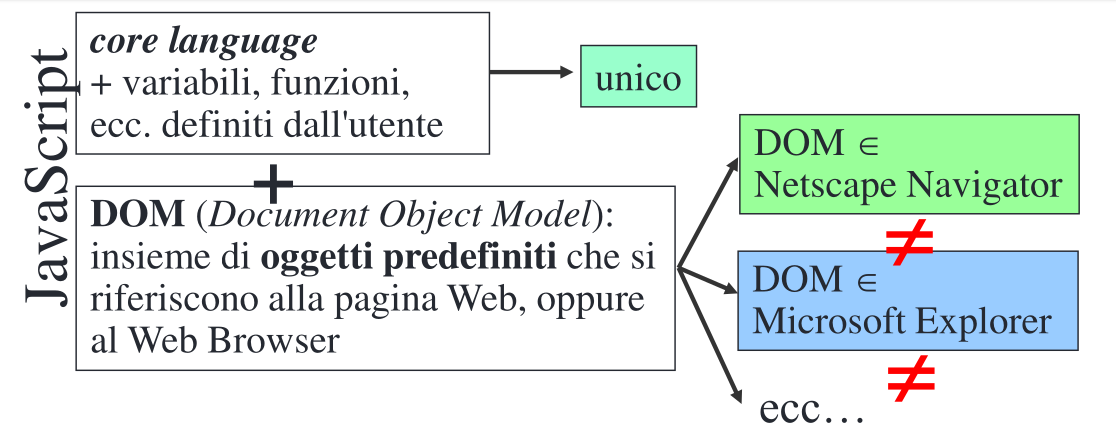
\includegraphics[width=0.5\textwidth]{Images/html_dom.png}
\end{figure}
JavaScript usa HTML DOM per modificare tutti gli elemetni di una pagina Web:
\begin{itemize}
    \item Quando una pagina è caricata il browser crea il DOM della pagina.
    \item La pagina è rappresentata come un albero.
    \item DOM è definito dal browser.
\end{itemize}
\subsection{Oggetti (DOM)}
Tramite il modello DOM a oggetti, Javascript può:
\begin{itemize}
    \item Cambiare tutti gli elementi e attributi HTML di una pagina.
    \item Cambiare tutti gli stili CSS.
    \item Rimuovere elementi e attributi HTML.
    \item Aggiungere elementi e attributi HTML.
    \item Reagire a eventi nella pagina.
    \item Creare nuovi eventi.
\end{itemize}
\subsubsection{Oggetti (DOM): Liste di oggetti}
Il DOM è organizzato seconod una gerarchia:
\begin{figure}[H]
    \centering
    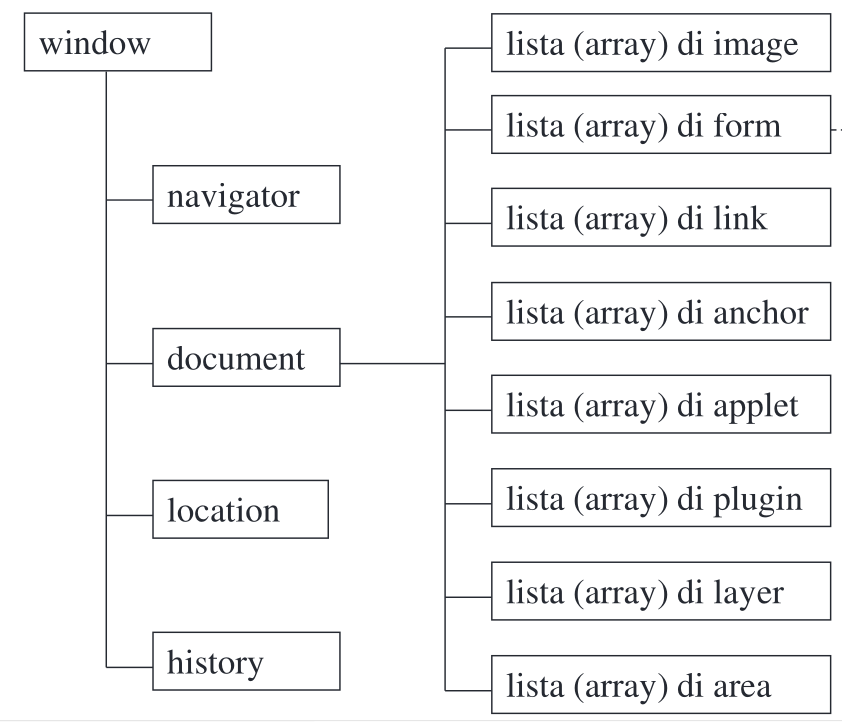
\includegraphics[width=0.5\textwidth]{Images/DOM_liste_oggetti.png}
\end{figure}
\begin{figure}[H]
    \centering
    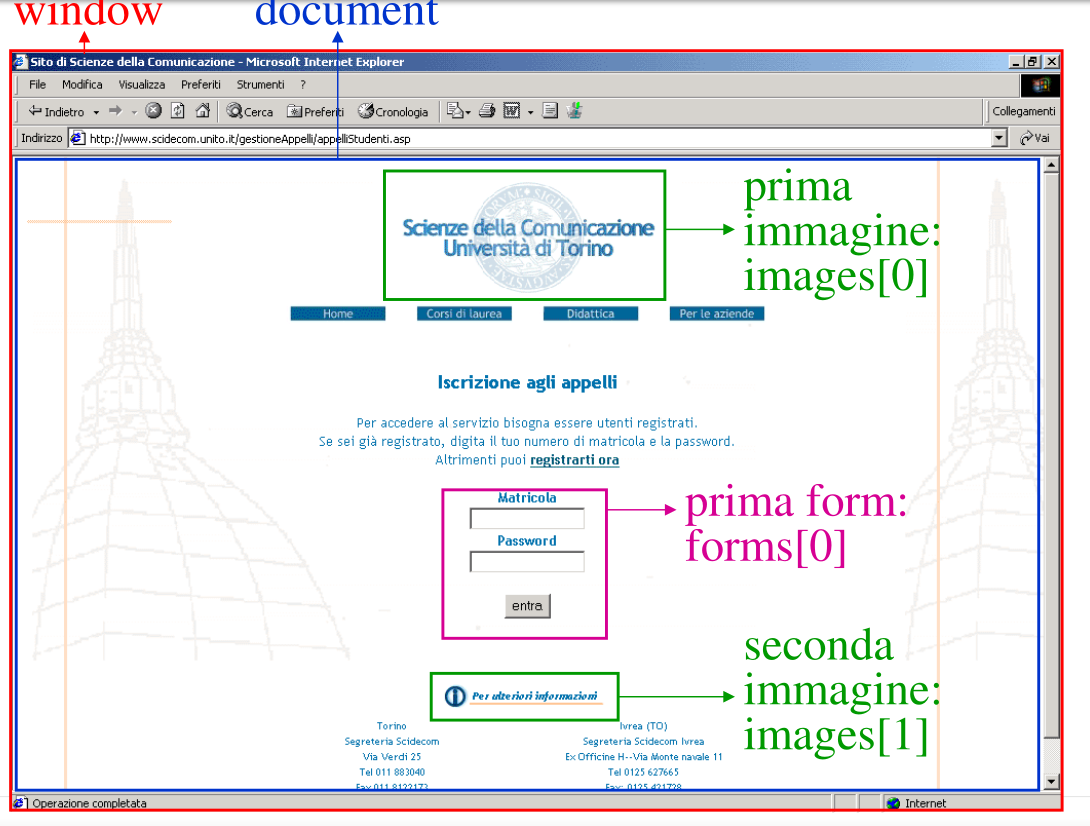
\includegraphics[width=0.5\textwidth]{Images/oggetti_DOM.png}
\end{figure}
\subsubsection{Oggetti (DOM): Window}
Windows (this) = la finestra corrente del browser. Figli dell'oggetto window:
\begin{itemize}
    \item navigator: il browser;
    \item document: il contenuto della finestra;
    \item location: informazioni sull'URL corrente;
    \item history: elendo degli URL visitati di recente.
\end{itemize}
\subsection{Window: componenti principale (estesi)}
\begin{itemize}
    \item self;
    \item windows;
    \item parent;
    \item top;
    \item navigator;
    \item frames (array);
    \item location;
    \item history;
    \item document;
\end{itemize}
\subsection{WIndow}
Radice della gerarchia DOM: rapprenta la finestra del browser e fornisce diversi metodi.
\\ Metodo Alert: \texttt{window.alert(messaggio)} propone una finestra di avviso con messaggio.
La funzione alert è usabile anche in un link e non restituisce nessun valore.
\\ Altri metodi:
\begin{itemize}
    \item confirm, che fa apparire una finestra di conferma con il messaggio dato: restituisce \texttt{true} o \texttt{false}.
    \item prompt, che fa apparire una finestra di dialogo per immettere un valore: resituisce il valore string.
\end{itemize}
\subsection{Document}
Rappresenta il documento corrente: il contenuto della oagina web attuale. I componenti principali di document sono:
\begin{itemize}
    \item forms (array): lista dei moduli (form) contenute nella pagina;
    \item elements (array di Buttons, Checkboc, ...)
    \item anchors (array);
    \item links (arrays);
    \item images (array): lista delle immagini contenute nella pagina;
    \item applets (array);
    \item ambeds (array).
\end{itemize}
Diversi metodi disponibili: \texttt{document.write} stampa un valore a video.
\subsection{Oggetti: proprietà e funzioni}
Un oggetto è una collezione di:
\begin{itemize}
    \item proprietà (variabili): sono a loro volta oggetti;
    \item funzioni (metodi, operazioni).
\end{itemize}
L'invocazione di una funzione apparentemente senza alcun oggetto si riferisce all'oggetto window. Un riferimento all'oggetto document non preceduto da un riferimento all'oggetto window, è equivalente al caso in cui document è preceduto da window (implicito).
\subsection{Accesso agli oggetti nella pagina}
Lista dei moduli contenuti in una pagina: \texttt{window.cocument.forms[i]}.
\\ Lista delle immagini contenute in una pagina: \texttt{window.document.images[i]}.
\\ I campi di testo sono oggetti dotati di nome posti all'interno di un oggetto form pure esso dotato di nome. Come tali sono referenziabili con la "dot notation": \texttt{documen.nomeform.nomeTextField}.
\\ Il campo di testo è caratterizzato dalla proprietà values.
\\ Esempio
\begin{lstlisting}[style=htmlstyle]
<FORM name="myform">
<INPUT type="text" name="cognome" size=20>
<INPUT type="button" name="bottone" value="Show"
onClick="alert(document.myform.cognome.value)">
</FORM>
\end{lstlisting}
Attributo NAME:
\begin{lstlisting}[style=htmlstyle]
<INPUT TYPE="text" NAME="codice_fiscale">
\end{lstlisting}
\begin{lstlisting}[language=JavaScript]
window.document.modulo.codice_fiscale.value=...
\end{lstlisting}
Metodo \texttt{getElementById(idname)}: ritorna l'elemento con uno specifico id. Ritorna \texttt{null} se non esiste l'elemento.
\begin{lstlisting}[style=htmlstyle]
<INPUT TYPE="text" ID="codice_fiscale">
\end{lstlisting}
\begin{lstlisting}[language=JavaScript]
window.document.getElementById("codice_fiscale").value=...
\end{lstlisting}
\subsection{Eventi}
I programmi JavaScript sono tipicamente "guidati dagli eventi" (event-driven). Gli eventi sono scatenati da azioni dell'utene sulla pagina Web: ogni volta che l'utente scrive qualcosa in una casella, preme un pulsante, ridimensiona una finestra ecc... genera un "evento".
\\ Un programma JavaScript deve contenere un gestore di eventi (event handler), che sia in grado di ricevere e interpretare le azioni dell'utente (eventi). Il DOM fornisce una serie di gestori di eventi predefiniti: l'accadere di un evento nella pagine Web mette automaticamente in azione il corrispondente gestore di eventi.
\begin{lstlisting}[style=htmlstyle]
<a href="#" onClick = "window.print()" >
\end{lstlisting}
Attributo \texttt{onClick}:evento click innesca il gestore. 
\\ Un'istruzione JavaScript può essere inserita all'interno di un tag HTML. In questi casi, il gestore di evento invocato farà riferimento al tag in cui si trova l'istruzione.
\\ Gli eventi intercettabili su un link: \texttt{onClick}, \texttt{onMouseOver}, \texttt{onMouseOut}. 
\\ Gli eventi intercettabili su una finestra: \texttt{onLoad}, \texttt{onUnload}, \texttt{onBlur}.
\subsection{Gestione eventi}
Per sfruttare il valore restituito da confirm, prompt o qualsiasi altra funzione JavaScript occorre inserire come valore dell'attributo onClick un programma JavaScript.
\begin{lstlisting}[language=JavaScript]
onClick = "x = prompt('Cognome e Nome:') ;
document.write(x)"
\end{lstlisting}
\subsubsection{Eventi (form)}
JavaScript permette di: intercettare eventi che "accadono" nei campi di un modulo e modificare i campi di un modulo.
\\ Un form contiene solitamente campi di testo e bottoni. Quando il bottone viene premuto è possibile invocare una funzione JavaScript.
\begin{lstlisting}[style=htmlstyle]
<FORM name="myform">
    <INPUT type="button" name="bottone"
    value="Premi qui"
    onClick = "alert('Mi hai premuto')" >
</FORM>
\end{lstlisting}
ALTERNATIVA: quando si preme il bottone, far scrivere il risultato di una funzione.
\begin{lstlisting}[style=htmlstyle]
<FORM name="myform"> 
    <INPUT type="button" name="bottone"
    value="Premi qui"
    onClick = "document.write(15)" >
</FORM>
\end{lstlisting}
Modifica di un campo del messaggio tramite proprietà \texttt{onMouseOver} e \texttt{onMouseOut}.
\begin{lstlisting}[style=htmlstyle]
    <DIV ALIGN="CENTER">
    <FORM NAME="modulo">
        <INPUT TYPE="text" NAME="over" VALUE="Il mouse e sopra
            la scritta1 o la scritta2?" size="50px">
    </FORM>
    <A HREF="" onMouseOver= "window.document.modulo.over.value='scritta1';"
    onmouseout="window.document.modulo.over.value='Il mouse e sopra la
    scritta1 o la scritta2?'">scritta1</A>
    ...
\end{lstlisting}
Selezionare/deselezionare le checkbox al click su un link/bottone:
\begin{figure}[H]
    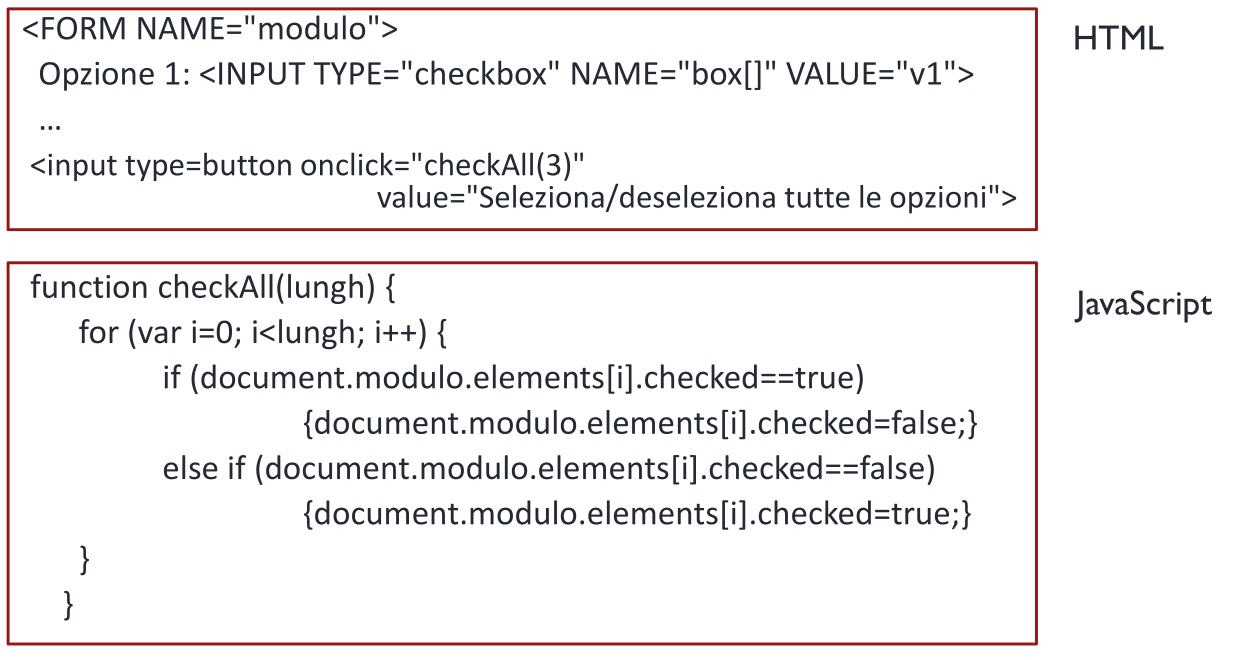
\includegraphics[width=0.5\textwidth]{Images/eventi_form_checkbox.png}
\end{figure}
Impostare dinamicamente le voci di un menu (a), intercettare il click del mouse sul pulsante di invio di un form e di conseguenza mostrare un alert (b).
\\ Menù:
\begin{lstlisting}[style=htmlstyle]
<FORM NAME="modulo" onSubmit=" warn(); return false;">
    <SELECT NAME="menu" id="menuid">
        <OPTION ID="fr" VALUE="inter">Inter</OPTION>
        <OPTION ID="pt" VALUE="milan">Milan</OPTION>
        <OPTION ID="st" VALUE="juve">Juve</OPTION>
    </SELECT>
    <INPUT TYPE="Submit" VALUE="OK">
</FORM>
\end{lstlisting}
\textcolor{red}{\textbf{return false} evita il refresh della pagina che avviene di default con il pulsante submit}.
Impostare dinamicamente le voci di un menu (a).
\begin{lstlisting}[style=htmlstyle]
<SCRIPT language="JavaScript">
    var nazione = prompt("Sei Italiano o Inglese?", "Italiano");
    if (nazione == "inglese") {
        window.document.modulo.menu.options[0].text="Chelsea";
        window.document.modulo.menu.options[1].text="Manchester United";
        window.document.modulo.menu.options[2].text="Manchester City";
        var select = document.getElementById('menuid');
        var opt = document.createElement('option');
        opt.id = "tt";
        opt.value = "liverpool";
        opt.innerHTML = "Liverpool";
        select.appendChild(opt);
}
</SCRIPT>
\end{lstlisting}
\end{document}

